\documentclass[a4paper,11pt]{article}
\pdfminorversion=4

\usepackage[english]{babel} % the new way
\usepackage[utf8]{inputenc}
\usepackage[T1]{fontenc}
\usepackage{lmodern}

\usepackage[left=2.5cm, right=2.5cm]{geometry}

% Palatino for rm and math | Helvetica for ss | Courier for tt
\usepackage{mathpazo} % math & rm
\linespread{1.05}        % Palatino needs more leading (space between lines)
\usepackage[scaled]{helvet} % ss
\usepackage{courier} % tt

% For language-specific hyphenations etc.
%\usepackage[english]{babel}
% For subfigures
\usepackage{subcaption}
% For nice links
%\usepackage{url}
% For playing with colors in tabular environments
\usepackage{colortbl}
% For math symbols, such as \nexists
\usepackage{amssymb}
% For more math symbols, such as \mapsfrom
\usepackage{stmaryrd}
% For advanced graphics
%% For including figures, graphicx.sty has been loaded in
%% elsarticle.cls. If you prefer to use the old commands
%% please give \usepackage{epsfig}
% For equations, arrays of equations, defining operator names, etc.
\usepackage{amsmath}
% For cursive math
%\usepackage{mathrsfs}
% For math symbols, such as \nexists
\usepackage{amssymb}
%% For math environments, such as "definition"
\usepackage{amsthm}
%\theoremstyle{definition}
%\newdefinition{definition}{Definition}[section]
%\newtheorem{theorem}{Theorem}[section]
% For enumerating the line numbers
\usepackage[left]{lineno}
% For side notes, missing figures and inline to-do's
\usepackage[textsize=scriptsize,backgroundcolor=orange!50]{todonotes}
% For specifying kewords and acronyms
\usepackage[nonumberlist,acronym,sanitize=none]{glossaries}
\glsdisablehyper
% For commenting out some parts of the text
\usepackage{comment}
% For building hyperlinks
\usepackage[pdftex, colorlinks=true, hyperfootnotes=true, hyperindex=true,
plainpages=false, pagebackref=false, pdfpagelabels=true, pdfstartview=FitH,
linkcolor=blue, citecolor=blue, urlcolor=blue,
bookmarks, bookmarksopen, bookmarksdepth=3]{hyperref}
\urlstyle{same}
\usepackage{etoolbox}
\makeatletter
\patchcmd\@combinedblfloats{\box\@outputbox}{\unvbox\@outputbox}{}{%
	\errmessage{\noexpand\@combinedblfloats could not be patched}%
}%
\makeatother

% For smart references
\usepackage{cleveref}
% To have "Figure 3(a)" in place of "Figure 3a" and  "Table 3(a)" in place of "Table 3a"
%\captionsetup[subfigure]{subrefformat=simple,labelformat=simple}
%    \renewcommand\thesubfigure{(\alph{subfigure})}
\captionsetup[subtable]{subrefformat=simple,labelformat=simple}
    \renewcommand\thesubtable{(\alph{subtable})}
\Crefname{algocf}{Algorithm}{Algorithms}
% TikZ/Pgf advanced graphics
\usepackage{tkz-base}
\usetikzlibrary{decorations.pathmorphing,trees,snakes,arrows,shapes,automata}
% To use inline and other fancy list-like environments (e.g., inparaenum)
\usepackage{paralist}
% To divide a text line into multiple columns
\usepackage{multicol}
% To create good-looking book-style tables
\usepackage{booktabs}
% To play around with list environments
\usepackage{enumitem}
% To create multirow cells in tables
\usepackage{multirow}
% To create rotated cells in tables
\usepackage{rotating}
% To specify properties of tables
\usepackage{array}
% To create enumerated lists, whose numbering is reversed
\usepackage{etaremune}
%% To make algorithmic nice-looking pseudocode
\usepackage[ruled,linesnumbered]{algorithm2e}
%% For creating side-notes
% \usepackage{marginnote}
% For superimposing symbols over one another within math env.
\usepackage{mathtools}
% For strange math symbols like \Dashv
\usepackage{mathabx}
% For LaTeX if/then statements
\usepackage{ifthen}
% For strike-through cancellations
\usepackage[normalem]{ulem}
%% The lineno packages adds line numbers. Start line numbering with
%% \begin{linenumbers}, end it with \end{linenumbers}. Or switch it on
%% for the whole article with \linenumbers.

\usepackage{booktabs}
% \usepackage{graphicx}
%\useunder{\uline}{\ul}{}
\usepackage{lscape}

\usepackage{lineno}
% For highlighted text
\usepackage{soul}
% To put table environments and co. side by side
%\usepackage{floatrow}
%\floatsetup[table]{style=plaintop}
% To add dummy text
\usepackage{lipsum}
% To have newlines in cells, with commands such as \makecell or \thead
\usepackage{makecell}
% To enable text protrusion
\usepackage[protrusion=true,expansion=true]{microtype}
%% PACKAGE TO INCLUDE A PDF FILE
\usepackage{pdfpages}
%% PACKAGE FOR THE HEADERS AND FOOTERS
\usepackage{fancyhdr}
%\usepackage[a-1a]{pdfx}
% theorem tools
\usepackage{thmtools}
%
\usepackage{float}
\RequirePackage{rotating}

\newcommand{\sidewaysheader}[1]{\begin{sideways}{#1}\end{sideways}}
\newcommand{\sidewaysheaderpar}[2]{\begin{sideways}\parbox{#1}{\centering #2}\end{sideways}}

\RequirePackage{paralist}

\newenvironment{iiilist}%
{\begin{inparaenum}[\itshape(i)\upshape]}%
{\end{inparaenum}}

\RequirePackage{colortbl}

\newcommand{\grayrow}{\rowcolor{gray!20}} %
\newcommand{\lightgrayrow}{\rowcolor{gray!10}} %
\newcommand{\graycell}{\cellcolor{gray!30}} %
\newcommand{\graytext}{\color[HTML]{606060}} %

\RequirePackage{todonotes}
\newcommand{\todoinline}[1]{\todo[inline]{#1}}

\newcommand\BackgroundPic{%
	\put(0,0){%
		\parbox[b][\paperheight]{\paperwidth}{%
			\vfill
			\centering
			%\includegraphics[width=\paperwidth,height=\paperheight,keepaspectratio]{background.pdf}%
			\vfill
}}}
\fancyhf{}% Clear all headers/footers
\fancyhead[R]{
\includegraphics{wu_top.png}}
\renewcommand{\headrulewidth}{0pt}% No header rule
\renewcommand{\footrulewidth}{0pt}% No footer rule
\fancyfoot[L]{\hspace*{0mm}
\includegraphics[scale=0.3]{logoDepartment.pdf}}

\newcommand*\rot{\rotatebox{90}}


\declaretheoremstyle[spaceabove=\topsep, spacebelow=\topsep,
headfont=\bfseries,
shaded={rulecolor=black, bgcolor={rgb}{1,1,1}},
numbered=no,
mdframed={
	leftmargin=2em,
	rightmargin=2em,
topline=false,
bottomline=false,
leftline=false,
rightline=false},
notefont=\mdseries,
bodyfont=\normalfont,
postheadspace=\newline,
headpunct=,
postheadhook=\leavevmode%
\interlinepenalty 10000%
\vskip-1.3\baselineskip%
\noindent{\rule{\textwidth}{1pt}}%
\interlinepenalty 10000%
\vskip0.3\baselineskip\noindent,
qed=\textcolor{black}{$\blacksquare$}]{example-style}

\declaretheorem[style=example-style]{example}
%
%%%%%%%%%%%%%%%%%%%%%%%%%%%%%%%%%%%%%%%%%%%%%%%%%%%%%%%%%%%%%%%%
% Acronyms / abbreviations
%%%%%%%%%%%%%%%%%%%%%%%%%%%%%%%%%%%%%%%%%%%%%%%%%%%%%%%%%%%%%%%%
%
\newacronym{bi}{BI}{Business Intelligence}
\newacronym[\glslongpluralkey={Business Processes}]{bp}{BP}{Business Process}
\newacronym{bpi}{BPI}{Business Process Intelligence}
\newacronym{bpm}{BPM}{Business Process Management}
\newacronym{bpmn}{BPMN}{Business Process Model and Notation}
\newacronym{bpms}{BPMS}{Business Process Management System}
\newacronym{dsr}{DSR}{Design Science Research}
\newacronym{ecg}{ECG}{event coupling graph}
\newacronym{epc}{EPC}{event-driven process chain}
\newacronym{ctd}{CTD}{computational theory discovery}
\newacronym{feds}{FEDS}{Framework for Evaluation in Design Science Research}
\newacronym{fmc}{FMC}{Fundamental Modeling Concepts}
\newacronym{gtm}{GTM}{grounded theory methodology}
\newacronym{ide}{IDE}{Integrated Development Environment}
\newacronym{it}{IT}{Information Technology}
\newacronym{its}{ITS}{Issue Tracking System}
\newacronym{kpi}{KPI}{Key Performance Indicator}
\newacronym{loc}{LOC}{lines of code}
\newacronym{msr}{MSR}{Mining Software Repositories}
\newacronym{nlp}{NLP}{Natural Language Processing} 
\newacronym{obda}{OBDA}{Ontology-based Data Access}
\newacronym{oss}{OSS}{Open-source Software}
\newacronym{owl}{OWL}{Web Ontology Language}
\newacronym{pn}{PN}{Petri net}
\newacronym{pm}{PM}{Process Mining}
\newacronym{ppi}{PPI}{Process Performance Indicator}
\newacronym{rbac}{RBAC}{role-based access-control} 
\newacronym{rup}{RUP}{Rational Unified Process}
\newacronym{soa}{SOA}{Service-Oriented Architecture}
\newacronym{svm}{SVM}{Support Vector Machine}
\newacronym{tm}{TM}{Text Mining}
\newacronym{tdt}{TDT}{Topic Detection and Tracking}
\newacronym{xes}{XES}{eXtensible Event Stream}
\newacronym{uml}{UML}{Unified Modeling Language}
\newacronym{vcs}{VCS}{Version Control System}
\newacronym{wf}{WF}{workflow}
\newacronym{wfms}{WfMS}{Workflow Management System}
%

%%%%%%%%%%%%%%%%%%%%%%%%%%%%%%%%%%%%%%%%%%%%%%%%%%%%%%%%%%%%%%%%
% Keywords
%%%%%%%%%%%%%%%%%%%%%%%%%%%%%%%%%%%%%%%%%%%%%%%%%%%%%%%%%%%%%%%%
%
% Automated discovery algorithms -------------------------------
%
\newglossaryentry{alpha}{name={$\alpha$},description={the $\alpha$ imperative process discovery algorithm}}
\newglossaryentry{alphap}{name={$\alpha+$},description={the $\alpha+$ imperative process discovery algorithm}}
\newglossaryentry{alphapp}{name={$\alpha++$},description={the $\alpha++$ imperative process discovery algorithm}}
\newglossaryentry{minerful}{name={MINERful},description={the MINERful declarative process discovery algorithm}}
\newglossaryentry{heuri}{name={Heuristic},description={the Heuristic Miner imperative process discovery algorithm}}
%
% Declarative process modelling --------------------------------
%
\newglossaryentry{declare}{name={\textsc{Declare}},description={the \textsc{Declare} declarative process modelling language}}
%
% Log, trace, event --------------------------------------------
%
% log alphabet
\def\LogAlph {\ensuremath{\mathcal{A}}}
\newglossaryentry{logalph}{
	name={log alphabet},description={process alphabet, as reflected in the log},%
	symbol={\LogAlph}}

% event universe
\def\EvtUniv {\ensuremath{\mathcal{E}}\xspace}
\newglossaryentry{evtuniv}{
	name={log alphabet},description={universe of events},%
	symbol={\LogAlph}}

%
% event
\def\Evt {\ensuremath{e}}
\newglossaryentry{evt}{
	name={event},description={a record of an instantaneous fact during the process enactment},%
	symbol={\EvtUniv}}

%
% perspective
\def\Perspective {\ensuremath{P}}\xspace
\newglossaryentry{persp}{
	name={event},description={a perspective},%
	symbol={\Perspective}}
%
% trace
\def\Trace {\ensuremath{\sigma}}\xspace
\newglossaryentry{evttrace}{
	name={trace},description={a sequence of \glsentrytext{event}s},%
	symbol={\Trace}}
%
% event log
\def\EvtLog {\ensuremath{L}}
\newglossaryentry{evtlog}{
	name={event log},description={a collection of \glsentrytext{trace}s},%
	symbol={\EvtLog}}

%
% event log
\def\AttrVal {\ensuremath{\#}}
\newglossaryentry{attrVal}{
	name={event log},description={a collection of attribute values},%
	symbol={\AttrVal}}

%
% task
\newglossaryentry{task}{%
	name={task},description={The non-divisible, elementary activity}}

% Pool of Events
\def\EventsPool {\ensuremath{PL}}
\newglossaryentry{eventspool}{
	name={Events Pool},description={A pool of events, where events are stored},%
	symbol={\EventsPool}}

%
% repetitiveness
\def\Repet {\ensuremath{Rep}}\xspace
\newglossaryentry{repetitiveness}{
	name={repetitiveness},description={fraction of uniqueness of an attribute},%
	symbol={\Repet}}



\begin{document}
\AddToShipoutPicture*{\BackgroundPic}
\thispagestyle{fancy}


{\vspace{2cm}~}
{\vspace{2cm}}

\bigskip\bigskip\bigskip\bigskip\bigskip\bigskip
%% SELECT BACHELOR OR MASTER THESIS
\vspace*{2cm}
{\noindent\Large Research Proposal\\}
\vspace*{1cm}
%% WRITE THE TITLE OF YOUR WORK
{\noindent\Huge\textbf{Mining software development projects\\}}

{\vspace*{2cm}}
%% WRITE THE NAME OF YOUR SUPERVISOR
{\noindent\large {\bf Author:} \\Saimir Bala, M.Sc.,  h1454574\\ Darwingasse 9/7, 1020 Vienna,   saimir.bala@wu.ac.at \\}

%%% WRITE THE NAME OF YOUR SUPERVISOR
%{\noindent\large {\bf Student number:} h1454574 \\ saimir.bala@wu.ac.at \\}

\bigskip
%% WRITE THE NAME OF YOUR SUPERVISOR
{\noindent\large {\bf Supervisor:} \\Prof. Dr. Jan Mendling, jan.mendling@wu.ac.at}

\bigskip

%% WRITE THE DATAE OF SUBMISSION
{\noindent\large {\bf Date of Submission:} \\ \today}

\bigskip\bigskip\bigskip\bigskip

{\em\noindent Institute for Information Business, Department of Information Systems and Operations\\ Vienna University of
Economics and Business, Welthandelsplatz 1, 1020 Vienna, Austria
}



\pagebreak

\begin{abstract}

Software development is a highly flexible endeavor. Yet, software development projects have specific requirements about quality, costs and time to deliver. Therefore, there is need for monitoring and controlling the software development process. 
%Both academia and industry have recognized the need for gathering more transparency about the development process. On the one hand, industry relies on specific tools for managing these processes, e.g., Jira, which allow to break down the development efforts into small tasks. Work done on these tasks is typically are easier to predict and trace. On the other hand, academia has seen the growth of several software engineering contributions that focus on using the data generated from tools used by developers to analyze their processes. 
This problem is tackled separately by three different disciplines, but existing approaches still fail at delivering process knowledge about software development that can be easily understood by managers.
%Main works in the software engineering area focus on the extraction of performance indicators, but they lack tacking into account the work-flow perspective that comprises the logical flow of activities. Therefore, approaches allow for obtaining a process perspective that is useful to managers are still lacking. 
This dissertation develops novel methods and algorithms that can be used to extract process knowledge from software development trace data. 
%This involves the handling of unstructured and semistructured data from software repositories, such as user comments during collaboration. 
As a result, it can be positioned as a bridge between the process mining discipline and the area of software engineering.
From a research point of view, the outcomes of this dissertation are a building block to further cross-fertilize research streams on process mining and software engineering. From a practical point of view, the outcomes of this dissertation allow the project manager to obtain a more familiar means of analysis on software development such as a process view.

\end{abstract}

\pagebreak
\tableofcontents
\pagebreak

\section{Introduction}
\label{sec:introduction}

Software development is a process that involves creativity. Yet, practical software development projects are executed with specific requirements on time, budget and quality. In order to fulfill these requirements the development process must be monitored. For example, it is important to know what type of work is being done at a certain moment in time and by whom. This is for instance the case for large development projects where coordination mechanisms emerge spontaneously among developers who want to contribute with their code.
These type of projects are difficult to control for several reasons. First, there is no clear understanding in how far a certain piece of code advances the current status of the project. Second, a piece of code written by a developer goes through different stages of code-review and it is difficult to predict whether it will ever be merged with the main source. Third, coordination of work may involve a large number of message exchanges among many developers in forums. Hence, it is not feasible to manually oversee what work is going on at a particular point in time. 

Literature has tackled this problem from different angles. In the area of process mining approaches exist that exploit event logs for abstracting a process model. In the area of software engineering, software repositories have been explicitly studied. These type of works provide several metrics that help with understanding various aspects of development. However, process mining approaches only work with event logs where activities are explicitly recorded in the log. This is not the case with software development where data is rather unstructured. Likewise, software engineering approaches lack a perspective about work patterns. 


This study addresses the discovery of work patterns from software development event data. To this end, it defines concepts to capture work from software repositories. This allows to construct several discovery techniques that provide information about different aspects of the development process. In this sense, this work provides a bridge between process mining and software engineering. The findings of this work enable project managers as well as software developers to raise transparency about the actual development based on facts. As a result, it enables both understanding the current status and monitoring for potentially unwanted patterns of work.

The rest of this proposal is organized as follows. \Cref{sec:problem-definition} describes the problem, the existing literature, and derives the solution requirements. \Cref{sec:state-of-field} provides background knowledge on the related fields of process mining, text mining, and mining software repositories. \Cref{sec:methods} explains the research method, the dataset and outlines the expected output of the thesis. \Cref{sec:preliminary-results} shows completed work so far. \Cref{sec:next-steps} outlines future steps towards the completion of this dissertation. \Cref{sec:dissertation-relevance} draws the implications for research and presents a dissemination plan.



%%Monitoring the process of software development is critical for software project managers. In practice, various project management approaches exist that guide the managers during the development of software projects. Usually these guidelines and methodologies stem from experience. However, in practical scenarios, every software development project is rarely carried out as planned. Therefore, empirical evidence given from the historical evolution of generated artifacts may provide important cues for checking the adherence of work to existing projects plans and milestones.

Software development projects are highly complex in nature. These projects include, among other aspects, the execution of an overall software development \emph{process}. In practice, various project management approaches exist that guide the managers during the development of software projects. Usually these guidelines and methodologies stem from experience. However, in practical scenarios, every software development endeavor is different. Projects may deviate from the plan for a number of reasons. Inadequate decisions made on the planing phased, bad management or improper resource allocation, to cite a few, may lead to situations where many ad-hoc interventions are required. In turn, this leads to unpredicted costs, missing milestone deadlines, unforeseen maintenance effort, and unsatisfactory quality. Therefore, monitoring the software development process is of utmost importance to project managers who want to deliver quality software in time and within budget limits.

Software process monitoring helps managers control the various aspects related to the development~\cite{Humphrey1995}. Especially, it is a scaffold for gaining transparency about the work being done at specific times. In particular, managers want to know the actual versus planned progress, what are the resources that actively participate in the work, whether resource-occupancy is high, what are actual tasks performed by the different organizational roles, what are typical patterns of work that lead to specific outcomes, etc. A starting point for analysis is the empirical evidence given from the historical evolution of artifacts (e.g., files, documentation, etc)
\todo{JM:I think this is not the problem, but the solution. Better: there is the potential ...}
. Therefore, there is the need for approaches that are able to extract process knowledge from the artifacts produced and stored in software repositories.

Literature has addressed several aspects about obtaining process insights from historical data. For instance, pieces of evidence stemming from information systems used by people to work on tasks have been used to obtain knowledge about actual time patterns 
\todo{JM: simplify sentences}
(e.g., when and how long do tasks take?) \cite{Lanz2014}, case perspective (e.g., what are the tasks and decisions?)~\cite{VanderAalst2005}, organizational structure (e.g., who works on which task?) \cite{Schonig2016b}, and flow perspective (e.g., how are tasks logically connected?) \cite{VanderAalst2007b}. These event data are the output of the different tools that are used by the project stakeholders. Examples are documentation, file changes in a \gls{vcs}, user comments in blogs, emails, task management in a \gls{its}.
% Hence, approaches that can handle semi-structured data (e.g. commits of a \gls{vcs}) are needed.
Nevertheless,
\todo{JM:Why "nevertheless"?}
 extant disciplines tackle different perspectives of mining the software development process. Contributions from the \gls{pm} discipline focus mainly on obtaining process models from well structured event logs~\cite{VanderAalst2016b}. Contributions from the \gls{msr} area focus on obtaining results from a software engineering point of view, e.g., code quality, code complexity, user analysis, functional dependencies, software visualization, etc~\cite{Pinzger2016}. 
\todo{JM:I think this is not yet well structured as an argument. Right, there are two levels: fields and existing techniques.Please refer back to how we write introductions.}
 Lastly, contributions from \gls{tm} focus on dealing with unstructured data. Hence, they are fundamental for analyzing user comments in software repositories~\cite{Aggarwal2015}. In order to obtain a better understanding of the real software development process these approaches should be combined. None of the above disciplines provides full-fledged approaches to obtain process knowledge from software development event data. Hence, there is the need for techniques that are able to work semi-structured data (e.g. commit in \gls{vcs} or logs) for providing knowledge about the perspectives of underlying process.

\todo[inline]{CC: If this is going to be the goal of the thesis, the existing gaps regarding the 4 perspectives have to be clearly described before. Why these perspectives? That should also be justified.}
With this dissertation, I aim at raising the transparency and objectiveness of software development practices by devising new algorithms and techniques that draws from the aforementioned disciplines. \todoinline{?}
 My research is guided by the question \textbf{RQ:} ``\emph{How can we make use of project event data to gather insights about the software development process that are informative to managers?}". 
To answer this question, new approaches are devised such as algorithms and methods for handling semi- and un-structured data which are not generated by a business process engine \todo{JM: no need to talk about process engines} (e.g., logs from \gls{vcs} and \gls{its}), following a \gls{dsr} paradigm. This includes transforming real data taken from the railway \todo{JM: why talking about railways here?} domain or from other real project \todo{JM: why "real data" from "real projects"? skip the "real"} into structured logs and further analyzing them. At the current stage, this thesis already contains a number of contributions that tackle the problem from different aspects. Among other research results, prototypes have been developed for helping managers to obtain high level cues on the projects. First, this thesis provides a tool to visualize the project history as a Gantt chart in order to check for anomalies of the amount of work that has been done on the different work-packages of the project. Second, this thesis devises a prototype to understand the \emph{de facto} roles of software project participants based on their comments in the \gls{vcs}. Third, this thesis provides a prototype to spot signs of work dependencies which may lead to inefficient practices. A fourth prototype is currently being developed in the context of ongoing work on mining pull requests from \gls{its}. With this last prototype, this thesis \todo{JM: this thesis does not yet exist. You mean research on this question?} addresses all four processes perspectives, i.e., time, case, organization, and control-flow.

The rest of this research proposal is organized as follows. \Cref{sec:problem-definition} describes the problem, the existing literature, and derives the solution requirements. \Cref{sec:state-of-field} provides background knowledge on the related fields of process mining, text mining, and mining software repositories. \Cref{sec:methods} explains the research method, the dataset and preliminary results in addressing the research requirements. \Cref{sec:expected-results} presents the expected results and future steps towards the completion of this dissertation. \Cref{sec:relevance} draws the implications for research and presents a dissemination plan.




%\section{Theoretical Framework and State of the Art}
%\label{sec:framework}
%
%What is the theoretical basic concept of the dissertation and in how far does it differ from other concepts? For all empirical studies it should be made clear: what are the working hypotheses and how do
%they differ from existing ones?
%
%Background on \gls{bpm}

\section{Problem Definition}
\label{sec:problem-definition}

Software development processes are highly complex endeavors that require the coordination of multiple resources. Compared to standard business processes, they present the following characteristics. First, 
%although there is a planning phase, 
they involve creativity when executing the tasks, i.e. there exists no strict process model that is followed by the developers to produce a new piece of code. Second, they are driven by methodologies, e.g., \gls{rup}, Scrum\footnote{\url{https://www.scrum.org}}, Waterfall, etc. These methodologies constitute guidelines and best practices for project success. Third, they typically make use of software tools such as \gls{its}, \gls{vcs} and \gls{ide}. Such tools typically record work activities into log files. Fourth, there is in general no process engine to control the execution. Rather than that, a project manager or a Scrum master has to make sure that tasks are made available to the respective resources. Fifth, it is not trivial to obtain high level information on performance measures such as the burn-down rate, which are resource bottlenecks, what are time requirements for certain tasks, what type of work is actually being done, and how productive are people working in certain tasks, etc. Hence, there is the need for algorithms and tools that help extracting this knowledge.

\begin{figure}
	\centering
	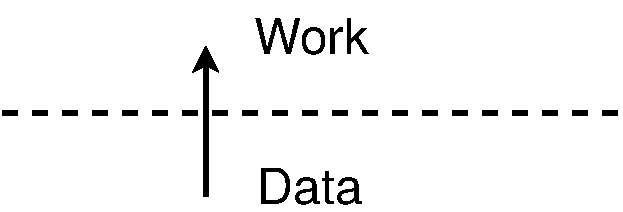
\includegraphics[width=0.5\linewidth]{figures/data-to-work}
	\caption{Illustration of the problem: work is reflected by available data}
	\label{fig:data-to-work}
\end{figure}


Software development processes fall into the category of \emph{project-oriented business processes} \cite{Bala2015}. 
That is, they are rather ad-hoc plans performed with limited resources and time, but with a clear goal: develop a software artifact. Unlike classic business processes which are best captured with notations such as Petri nets and \gls{bpmn}, software development processes are more akin to one-time plans, which are usually captured by models such as Gantt and PERT diagrams. The following example captures the essence of a typical software development process in practice, such as for instance in Google LLC~\cite{Henderson2017}.


\begin{quote}
A new software version or feature needs to be developed. Unquestionably, Google has know-how on software development. However, before running straight into the development phase, the company first makes sure to gather and properly formulate all the requirements. In a Scrum scenario these requirements would be written down as user stories. At a later stage, the project manager needs to plan the time and resources allocated to the respond to project deadlines. He can go through the list of requirements that need to be implemented and assign to an effort estimation value to each of them. With the plan done, the development phase can commence. During the development phase, resources address the task in a creative way, choosing the order of the tasks according to their own knowledge and expertise, until eventually all the tasks are terminated. Every time a resource wants to save their progress issue a so-called \emph{commit} command which creates a new version of the modified files on the \gls{vcs}. Likewise, every time a certain task (which may be worked carried out through by different commits) is completed, it is marked as done in the \gls{its}. Both the commits and the tasks can be commented by the users, respectively to document the changes and raise a discussion for better understanding the task goals.
\end{quote}

Several tools are used by software project participants to support their work. Therefore, traces about the overall process are typically available under different repositories and artifacts, e.g., spreadsheets, word processor documents, programming languages files, emails, etc. This makes it cumbersome to obtain knowledge about the overall business process through manual inspection. Also, it is a challenge to automatically \emph{extract} work information from unstructured data such as user comments when working on tasks. For instance, existing solutions (e.g., process mining algorithms) are not able to provide informative results when the data is not available as a structured single event log where activities are explicitly labeled. Likewise, other software tools (e.g. GitHub) limit themselves at providing only process-unaware statistical information (e.g., number of commits in a file).

%Therefore, the overall challenge is to understand which are important events that track development work in the repository. 


While obtaining an overarching view on software development is challenging, there are still repositories that we can be exploited to obtain process knowledge. One tool that provides important traces of the development work is \gls{vcs}. This tool is used to keep track of the different versions of files created by users and to manage their collaboration. Not only they allow to keep track of the different versions, but also allow users to associate a textual comment that describe the changes made. Therefore, a new version of a particular file is created as the result of an activity done by a user. The evolution of these versions, along with information about the users and their comments can be retrieved from these type of tools in the form of semi-structured event logs. It is then a challenge how to discover the business process from events (e.g., lines of code changed, comments, user information) present in these logs.

%
%\todo{JM: I think you have to develop much more clearly how it is difficult to extract certain pieces of information from version control systems.} 

%An important dimension of the software development process is the work dimension, i.e. the process. This perspective is particularly interesting to project managers. One of their goal is to know whether the planning phase was realistic with respect to the development efforts. Existing software repositories allow for many ways to access their log files. These log files offer factual information about actions done by the process participants to change the repository state.

\begin{figure}[h]
	\centering
	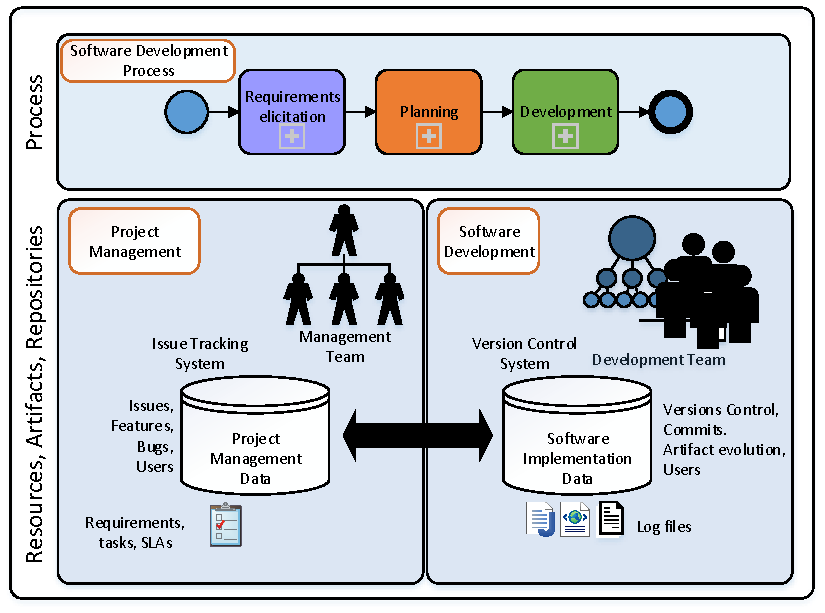
\includegraphics[width=0.7\linewidth]{figures/big-picture}
	\caption{Software development scenario with two repositories used for project management and software development, respectively.}
	\label{fig:big-picture}
\end{figure}

\Cref{fig:big-picture} illustrates such problem scenario. Software development relies on tools like \gls{its} (e.g., JIRA, GitHub Issues) and \gls{vcs} (e.g. Subversion, Git). One the one hand, \gls{its} is used for tracking the project management aspect. This aspect offers plan related information, such as issues, features, bugs, text, planned and executed tasks, timestamps, stories, and effort estimation (e.g., story points in JIRA).
On the other hand, \gls{vcs} offers information about work traces, such as versions of the artifacts, number and content of commits done by developers, artifacts evolution, users and their comments, and timestamps of each action. 
% Please add the following required packages to your document preamble:
% \usepackage{booktabs}
% \usepackage{graphicx}
% \usepackage[normalem]{ulem}
% \useunder{\uline}{\ul}{}
%\vspace*{-.5cm}
\newcommand{\rowsep}{\vspace*{2pt}}
%\newcommand{\colsep}{\hspace*{52pt}}
\begin{table}[h]
	\caption{An excerpt of a VCS log data}
	\label{tab:vcs-log-data}
	\setlength{\tabcolsep}{6pt}
%	\setlength\belowcaptionskip{-20pt}
\centering
\resizebox{.8\textwidth}{!}{%
%\begin{tabular}{@{ }cm{.7cm}m{2cm}m{4.8cm}m{7cm}@{ }}
\begin{tabular}{@{~~}cm{1.2cm}m{2cm}m{3.6cm}m{7.5cm}@{}}
%\toprule
\textbf{Id} & \textbf{Resource } & \textbf{ Date}                          & \textbf{Comment}                          & \textbf{Diff}                                                                                                                                                                                                                                                                                   \\ \midrule 
%\rowcolor{lightgray}
1          & John    & 2017-01-31 12:16:30 & Create readme file                   & \begin{tabular}[c]{@{}l@{}}diff --git a/README.md b/README.md\\ @@ -0,0 +1 @@\\+\# StoryMiningSoftwareRepositories\end{tabular}                                                                                                                                                          \\ \rowcolor{lightgray}
2          & Mary    & 2017-02-01 10:13:51 & Add a license                   & \rowsep \begin{tabular}[c]{@{}l@{}}diff --git a/README b/README\\ @@ -1,0 +2,3 @@\\ +The MIT License (MIT)\\ +\\ +Copyright (c) 2015 Mary+\end{tabular}                                                                                                                                     \\
%\rowcolor{lightgray} 
3          & Paul    & 2017-02-02 16:10:22 & Updated the requirements.               & \rowsep \begin{tabular}[c]{@{}l@{}}diff --git a/README.md b/README.md\\ @@ -1,4 +1,5 @@ \\ + \# string 1, string 2, string 3\\ \\ diff --git a/requirements.txt b/requirements.txt\\ @@ -0,0 +1 @@\\ +The software must solve the problems\end{tabular} \\ \rowcolor{lightgray}
4          & Paul    & 2017-02-02 15:00:02 & Implement new requirements & \rowsep \begin{tabular}[c]{@{}l@{}}diff --git a/model.java b/model.java\\ @@ -1,9 +1,10 @@ \\ {+public static methodA()\{int newVal=0;}\\ @@ -21,10 +23,11 @@\\ + "1/0",,"0/0",\\ \\ diff --git a/test.java b/test.java\\ @@ -0,0 +1,2 @@\\ +//test method A\\ +testMethodA()\end{tabular}  \\ \bottomrule
\end{tabular}%
}
\end{table} 


Although different technologies exist in practice (e.g., Subversion, Mercurial, Git), the information contained in the logs can be roughly summarized by \Cref{tab:vcs-log-data}. The table displays an excerpt of a \gls{vcs} log, i.e., a set of user commits, after having extracted and structured the data according to five attributes. The semantics of the  attributes is a follows: 
\begin{inparaenum}[\itshape i)]
	\item \emph{Id} is a unique identifier;
	\item \emph{Resource} is the resource that issued the commit;
	\item \emph{Date} is a timestamp associated to the time and date the commit was stored in the system;
	\item \emph{Comment} is a user comment on the changes made;
	\item \emph{Diff} is low-level information on the difference between the current and the previous version, for each file.
\end{inparaenum} 
Likewise, information about issues from \gls{its} can be extracted and presented in a tabular way. In this case, other attributes are more important. These attributes can be, for example, the status of issues and the conversations that take place around them. %As the relation between \gls{its} and \gls{vcs} about requirements-implementation, we can narrow down our research question to the following. \emph{\textbf{RQ:} How does the specification of user stories influence software development work?} 
%In the more specific case, \gls{vcs} logs consist of an ordered set of \emph{commits} bearing information about users, files, timestamp, comments and type of change that were stored at particular moment in time. \Gls{its} typically come with richer information, most importantly they inform about users, task, type of task (e.g., bug, new feature, requirement, etc), timestamps, related issues, etc. 
%Many types of analyses can be performed on such feature rich data once they have been properly correlated and structured. 
Hence, studying the co-evolution of these two repositories can help extracting relevant knowledge about the software development process. 

More precisely this work wants to answer to the following research question. \textbf{RQ}: \emph{How can we make use of project event data to gather insights about the software development process that are informative to managers?} 
Because the project managers can benefit from a process view to better analyze hidden aspects of the software development process, this work takes a process mining stance on the problem. Therefore, the main research question is broken down into the following four subquestions. Each of them addresses \textbf{RQ} with respect to the four perspectives of a process that are useful to discover the event data~\cite{VanderAalst2016b}.

%In the light of the above considerations, we derive the following requirements for extending process mining towards the analysis of software repositories.
%Owing to \gls{pm} literature, the research question (\textbf{RQ}) can be further broken down to the four process mining perspectives. 
%From here, we derive the four fundamental requirements that satisfy \gls{msd}.

\begin{description}
	\item[RQ1. Mining the time perspective.] \emph{How can we use project event data to extract information about the temporal aspect of activities?} For example, an answer to this question would look like: the development activity has a duration of 2 weeks on average, the average time of task creation is 15 minutes, etc. 
	
	\item[RQ2. Mining the case perspective.] \emph{How can we use project event data to extract information about the case perspective?} For example, an answer to this question would look like: all the bugs are solved in a 3 steps iteration, or a quality piece of code takes a conversation with 3 people and is successfully merged into the main branch after 1 week, etc.
	
	\item[RQ3. Mining the organizational perspective.] \emph{How can we use project event data to extract information about the organizational perspective?} For example, an answer to this question would look like: the software development is carried out by a team of 4 people, the actual user roles in the company are developer and tester, etc.
	
	\item[RQ4. Mining the control-flow perspective.] \emph{How can we use project event data to extract information about the control-flow perspective?} For example, an answer to this question would look like: the testing is always done before development, or while new features are worked on, also new requirements are created, etc. Note that, differently from \textbf{RQ1} this question focuses on the logical connection and order of activities.
	
\end{description}


\section{State of the Art}
\label{sec:state-of-field}
%\subsection{Literature review}
The described problem has been partially addressed in three research areas:
\begin{inparaenum}[\itshape i)]
	\item \gls{pm};
	\item \gls{msr}; and
	\item \gls{tm}.
\end{inparaenum}
The following sections introduce these fields along with their contribution to the research question and limitations. 

\subsection{Process Mining}
\label{sec:process-mining}

\subsubsection{Description of the field}

Process mining is a discipline that emerged in the last decade. The goal of this discipline is to provide fact-based insights and support process improvement. On a broader context, process mining can be considered as the missing link between traditional model-based process analysis and data driven techniques such as data mining and machine learning~\cite{VanderAalst2016b}. Compared to existing \gls{bi} technologies, process mining techniques go beyond the calculation of simple \glspl{kpi}. Instead, by building on model-driven approaches, they provide means to gain transparency on several aspects of the end-to-end business process. More specifically process mining techniques can infer models from event logs, which inform about the diverse aspects of a business process.
As defined in~\cite{VanderAalst2016b}, main \emph{perspectives}\footnote{Note that the different perspectives are partially overlapping. Nevertheless, a good reason to adopt them is because they are widely used in the \gls{bpm} community.} of a business process are the following. 

\begin{itemize}
	
	\item The \emph{time perspective} aims at analyzing time and frequency of process events. The focus is to use time information for performance analysis, such as bottlenecks, resource utilization, prediction of workload, remaining running time of process instances, etc. Note that the output of this method is not necessarily a process model, but rather metrics that can be integrated with process models.
	
	\item The \emph{case perspective} aims at identifying properties of process cases. A process case is one execution of a process from start to end, e.g. from the moment a customer order a product to its delivery. However, there can be other ways to determine cases, e.g., the evolution of a data artifact, such a for instance the fulfillment of monthly report of the orders. 
	
	\item The \emph{organizational perspective} aims at analyzing the event log to gain transparency on the resources involved in the process. The focus of this perspective is to help understanding which are the people and systems in the process and how are they related in terms of roles, hierarchy, handover of work, privileges, access-control, social network, etc.
	
	\item The \emph{control-flow perspective} aims at analyzing the different variations of the process, i.e., in which order its constituting activities are carried out in real life. The focus of this perspective is on characterizing all possible process paths. Outcome typically results in models expressed as Petri nets, \gls{bpmn}, \gls{epc}, \gls{uml}, etc.	
	
\end{itemize}


%These aspects can be, for example, related to the control flow (i.e., the various steps for used by the company for generating value), resources (i.e., handover of work among the different process participants), activities (i.e., how the work is broken down into several tasks), and data (i.e., which artifacts are produced and consumed by the process). 

Process mining is becoming and established field with considerable number of algorithms from academia and a many industry tools such as Celonis\footnote{\url{https://www.celonis.com}}, Disco\footnote{\url{https://fluxicon.com/disco}}, minit\footnote{\url{https://www.minit.io}}, LANA Process Mining\footnote{\url{https://lana-labs.com/en}} and many more. 
Mining algorithms are developed every year to deal to mine not only process workflow, but also other perspectives, i.e. organizational, data, etc. \Cref{fig:process-mining} illustrates process mining research and how it relates event data from real world and business process models.
There are three types of process mining, namely \begin{inparaenum}[\itshape i)]
	\item process discovery;
	\item conformance checking; and
	\item enhancement.
\end{inparaenum} This proposal focuses more on the discovery part, i.e., take an event log as an input and abstract process patterns from it. 


%\begin{description}
%	
%	\item[Process discovery.] This type of process mining is concerned with the inference of process models from event logs. Process discovery algorithms are typically unsupervised techniques that produce models in various notations such as Petri nets, \gls{bpmn}, \gls{epc}, etc. A example of a process discovery algorithm is the so-called $\alpha$-algorithm~\cite{VanderAalst2004}.
%	
%	\item[Conformance checking.] This type of process mining compares the model and the log of the same process. The goal is to verify if the reality as recorded in the event log corresponds to the plan as defined by the model. Possible deviations are quantified making it possible to obtain important cues about bad performance in case the model is prescriptive or noncompliance in case the model is normative. 
%	
%	\item[Enhancement.] This type for process mining is focused on improving the existing process model by using information from past executions recorded in the log. Differently from conformance, the goal is to go beyond measuring the misalignment but actually correcting the process model. Main types of corrections are \emph{repair}, where a process model is repaired to better explain the data from the log, and \emph{extension}, where a new information is added to the process model that is found in the log, e.g., labeling activities with the resource names, labeling sequence flows with durations, and so on.
%	
%\end{description}


\begin{figure}
	\centering
	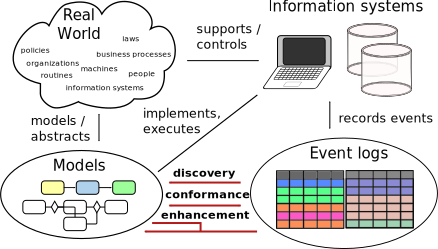
\includegraphics[width=0.6\linewidth]{figures/process-mining-big-picture}
	\caption{The process mining framework Adapted from \cite{VanderAalst2016b}.}
	\label{fig:process-mining}
\end{figure}



%Nevertheless, process mining algorithms work with structured data~\cite{van2005prom, Verbeek2011}. 

\subsubsection{Contribution to the research questions} 

Several works in the area of \gls{pm} have tackled the problem by transforming it into a \gls{pm} problem. 
%These works enrich \gls{vcs} log data with case and activity information, and then use process mining to discover a model. In this category, Kindler et al.~\cite{kindler2006activity,kindler2006incremental} can discover a Petri net from a structured and enriched version control log. This approach was further improved by Rubin et al.~\cite{rubin2007process} and a ProM\footnote{\url{http://www.promtools.org}} plug-in was provided. Poncin et al.~\cite{Poncin2011a} provide the FRASR framework for preprocessing software repositories such that they can be used in ProM. Song et al.~\cite{Song2007} help addressing the time perspective by mining a dotted chart.
Consequently, approaches have been developed to preprocess VCS data such that process mining techniques can be applied, and hence, a business process can be derived from the log data.
In this group, Kindler et al. \cite{kindler2006activity,kindler2006incremental} developed an algorithm for extracting software processes that are mapped to Petri Nets. Activities, which are not explicit in the logs, are discovered from their input and output artifacts. However, strong assumptions are made on the filenames as well as on the software process lifecycle. %(always design, code, review, testres). Activities (which are not explicit in the logs, like in our case) are discovered from their input and output artifacts. Here defined as triples $<I,O,R>$ where I=input, O=Output, R=resouce who perfomed it.
Rubin et al. in \cite{rubin2007process} addressed the problem of engineering processes that are not well documented and are usually unstructured. They provided a bridge from Kindler et al.'s approach to ProM \cite{van2005prom} in order to mine different process perspectives, such as performance social network analyses. %but not from a project point of view.
Rubin et al. \cite{rubin2014agile} applied process mining to the touristic industry and obtained user processes from web client logs pursuing the goal of improving the software system by analyzing the underlying process.
Poncin et al. \cite{Poncin2011a} developed the FRASR framework for preprocessing software repositories to transform the VCS data to logs that conform to the process mining event log meta model~\cite{van2005meta} as utilized in ProM \cite{van2005prom}.
However, these approaches disregard the single-instance nature of project-oriented business processes and treat them as procedures that can be repeated over time.

Process mining techniques are related to all the research questions of this thesis. Especially, they help with addressing \textbf{RQ4}, i.e. finding the control flow of software development activities.

\subsubsection{Limitations} 
While providing interesting insights, these contributions leave out many important aspects of software development projects, such as trying to understand whether the process was done according to the organization plan. Especially, they are limited to either simply display one perspective of the process~\cite{Song2007} or transform the events from software repositories into the standard \gls{xes} format which can be mined by tools like ProM. In this case, existing methods only take into account high level information (such as the type of file) to label events accordingly. Textual information is also taken into account \cite{rubin2007process} but often limited to use of a dictionary for identifying keywords. Moreover, fine granular information on the amount of change and the comments of commit messages have not been exploited enough by existing literature.

This works aims to use the strengths of process mining techniques on discovering informative models. At the same time, it aims to go beyond the current limitations of these techniques to handle fine granular (e.g., amount of changes) and unstructured data (e.g. user comments).
%The challenge is then how to extract  \gls{vcs} log data is semi-structured and not always can be related to the standard XES~\cite{Verbeek2011} required by process mining algorithms.


\subsection{Text Mining}
\label{sec:text-mining}


\subsubsection{Description of the field} 

Text mining refers to the process of deriving information from natural language text. It relates to data mining in the aspect that both strive to extract meaningful information from raw data. However, data mining is characterized as the extraction of implicit, previously unknown, and potentially useful information from data, whereas with text mining the information to be extracted is clearly and explicitly stated in the text~\cite{Witten2004}. 
Text mining can be regarded as going beyond information access to further help users analyze and digest information and facilitate decision making. There are also many applications of text mining where the primary goal is to analyze and discover any interesting patterns, including trends and outliers in text data.
Although text mining is mostly about \gls{nlp}~\cite{jurafsky2014speech}, it embraces also applications that go beyond. For example, it analyzes linkage structures such as the citations in the academic literature and hyperlinks in the Web literature, both useful sources of information that lie outside the traditional domain of \gls{nlp}. 

%The main types of text mining are the following.
%
%%\Cref{tab:text-mining-overview} gives a compact overview on the types of text mining and some example references.
%%
%%\begin{table}[!h]
\centering
\caption{Overview on text mining types}
\label{tab:text-mining-overview}
\vspace{5pt}
%\resizebox{\textwidth}{!}{
\begin{tabular}{m{4cm}m{5cm}m{4cm}}
\toprule
\textbf{Type}                         & \textbf{Task}                                                                                                                   & \textbf{References}                                                                                           \\ \midrule
Information extraction       & Filling in templates from natural language text                                                                        & \cite{cowie1996information}, \cite{mooney1999relational}, \cite{seymore1999learning}, \cite{banko2007open} \\ %\midrule
Topic detection and tracking & Finding and following new events in a stream                                                                           & \cite{Allan1998}, \cite{wayne2000multilingual}                                                  \\ %\midrule
Summarization                & Reducing the content obtained from text documents, still keeping the topic                                             & \cite{aggarwal2012mining}, \cite{gupta2009survey}                                                    \\ %\midrule
Categorization               & Identifying the main themes of a document                                                                              & \cite{sebastiani2002machine}, \cite{joachims1998text}                                                \\ %\midrule
Clustering                   & Group similar documents by predefined topics                                                                           & \cite{zhao2001criterion}, \cite{fung2003hierarchical}, \cite{aggarwal2012mining}                     \\ %\midrule
Concept Linkage              & Connect related documents by identifying their shared concepts                                                         & \cite{maedche2000mining}, \cite{fan2006tapping}, \cite{gupta2009survey}                             \\ %\midrule
Information visualization    & Visualizing large textual sources                                                                                      & \cite{wong1999visualizing}, \cite{Mostafa2013}                                                       \\ %\midrule
Question answering           & Automatically answer questions posed by humans                                                                         & \cite{katz1997sentence}, \cite{kwok2001scaling}, \cite{aggarwal2012mining}                           \\ %\midrule
Association rule mining      & Study the relationships and implications among topics or descriptive concepts that are used to characterize a corpus & \cite{agrawal1993mining}, \cite{agrawal1994fast}, \cite{hu2010}                                      \\ \bottomrule
\end{tabular}
%}
\end{table}
%
%\begin{description}
%	\item[Information extraction.] 
%%	Information extraction is used to refer to the task of filling in templates from natural language text. The goal is to extract from the documents (which may be in a variety of languages) salient facts about prespecified types of events, entities or relationships. These facts are then usually entered automatically into a database, which may then be used to analyze the data for trends, to give a natural language summary, or simply to serve for on-line access. Traditional information extraction techniques~\cite{cowie1996information,mooney1999relational} leverage on rule-based systems that match predefined linguistic patterns. More recently, work on named entity recognition uses statistical machine learning methods~\cite{seymore1999learning}. A tool that uses unsupervised learning can be found in \cite{banko2007open}.
%	It is the task of filling in templates from natural language text. The goal is to extract from the documents (which may be in a variety of languages) salient facts about prespecified types of events, entities or relationships. They can be used to analyze the data for trends, to give a natural language summary, or simply to serve for on-line access. Typical examples can be found in~\cite{cowie1996information,mooney1999relational,seymore1999learning,banko2007open}.
%	
%	\item[Topic detection and tracking.] 
%%	\Gls{tdt} was a DARPA-sponsored initiative to investigate on finding and following new events in a stream of broadcast news stories. The \gls{tdt} problem consists of three major tasks: (1) \emph{segmenting} a stream of data, especially recognized speech, into distinct stories; (2) \emph{identifying} those news stories that are the first to discuss a new event occurring in the news; and (3) given a small number of sample news stories about an event, \emph{finding} all \emph{following} stories in the stream.
%%	The work of \cite{allan2002introduction} has formally defined this problem and proposed the initial set of algorithms for the task. Main subtasks of TDT, as identified in \cite{wayne2000multilingual} are 
%%	(i) finding topically homogeneous regions (segmentation); (ii) finding additional stories about a given topic (tracking); (iii) detecting and threading together new topics (detection); (iv) Detecting new topics (first story detection); and (v) Deciding whether stories are on the same topic (linking). An example of a real-world TDT system is Google Alerts\footnote{\url{https://www.google.com/alerts}}.
%	The \gls{tdt} problem consists of three major tasks: (1) \emph{segmenting} a stream of data, especially recognized speech, into distinct stories; (2) \emph{identifying} those news stories that are the first to discuss a new event occurring in the news; and (3) given a small number of sample news stories about an event, \emph{finding} all \emph{following} stories in the stream.
%	Typical examples can be found in~\cite{wayne2000multilingual,allan2002introduction}.
%	%	The work of \cite{allan2002introduction} has formally defined this problem and proposed the initial set of algorithms for the task. Main subtasks of TDT, as identified in \cite{wayne2000multilingual} are 
%	%	(i) finding topically homogeneous regions (segmentation); (ii) finding additional stories about a given topic (tracking); (iii) detecting and threading together new topics (detection); (iv) Detecting new topics (first story detection); and (v) Deciding whether stories are on the same topic (linking). An example of a real-world TDT system is Google Alerts\footnote{\url{https://www.google.com/alerts}}.
%	
%	\item[Summarization.] 
%%	Summarization is the task of reducing the content obtained from text documents, still keeping a brief overview on a topic that they treat. Summarization techniques generally fall into two categories \cite{Aggarwal2015}. In extractive summarization, a summary consists of information units extracted from the original text; in contrast, in abstractive summarization, a summary may contain {\textquotedblleft synthesized\textquotedblright} information units that may not necessarily occur in the text document. An automatic summarization process can be divided into three steps \cite{gupta2009survey}: (1) the \emph{preprocessing} step where a structured representation of the original text is obtained; (2) the \emph{processing} step where an algorithm must transform the text structure into a summary structure; and (3) the \emph{generation} step where the final summary is obtained from the summary structure. 
%%	A plethora of text summarization tools can be found online. A few examples are the open source libraries such Open Text Summarizer\footnote{\url{https://www.splitbrain.org/services/ots}}, Sumplify\footnote{\url{http://sumplify.com/}} and Online summarize tool\footnote{\url{http://www.tools4noobs.com/summarize/}}.
%Summarization is the task of reducing the content obtained from text documents, still keeping a brief overview on a topic that they treat. Typical examples of can be found in~\cite{gupta2009survey,Aggarwal2015}. Some open source libraries are Open Text Summarizer\footnote{\url{https://www.splitbrain.org/services/ots}}, Sumplify\footnote{\url{http://sumplify.com/}} and Online summarize tool\footnote{\url{http://www.tools4noobs.com/summarize/}}.
%	
%	\item[Categorization.] 
%%	Categorization aims at identifying the main themes of a document. This translates into assigning natural language documents to predefined categories according to their content~\cite{sebastiani2002machine}. Categorization often relies on a thesaurus for which topics are predefined, and relationships are identified by looking for broad terms, narrower terms, synonyms, and related terms. \Glspl{svm} are used to automatically learn text classifiers from examples~\cite{joachims1998text}. Categorization tools usually rank documents according to how much of their content fits in a particular topic. 
%%	
%	Categorization aims at assigning natural language documents to predefined categories according to their content. 
%%	Categorization often relies on a thesaurus for which topics are predefined, and relationships are identified by looking for broad terms, narrower terms, synonyms, and related terms. 
%	\Glspl{svm} are used to automatically learn text classifiers from examples. Typical examples can be found in~\cite{joachims1998text,sebastiani2002machine}.
%%	Categorization tools usually rank documents according to how much of their content fits in a particular topic. 
%	
%	\item[Clustering.] 
%%	Clustering is a technique used to group similar documents, but it differs from categorization in that documents are clustered on the fly instead of through predefined topics. Documents can also appear in multiple subtopics, ensuring that useful documents are not omitted from the search results. A basic clustering algorithm creates a vector of topics for each document and measures the weights of how the document fits into each cluster. A survey of clustering algorithms can be found in \cite{Aggarwal2015}. 
%	Clustering is a technique used to group similar documents, but it differs from categorization in that documents are clustered on the fly instead of through predefined topics. 
%%	Documents can also appear in multiple subtopics, ensuring that useful documents are not omitted from the search results. A basic clustering algorithm creates a vector of topics for each document and measures the weights of how the document fits into each cluster. 
%A literature review of clustering algorithms can be found in \cite{Aggarwal2015}. 
%	
%	\item[Concept Linkage.] 
%%	Concept-linkage tools connect related documents by identifying their shared concepts, helping users find information they perhaps would not have found through traditional search methods~\cite{gupta2009survey}. It promotes browsing for information rather than searching for it. For example, a text mining software solution may easily identify a transitive closure in a set of topics \{X, Y, Z\}, i.e., a link between X and Y, a link between Y and Z, %. But the text mining tool could also detect a potential 	and a link between X and Z. %(i.e. transitive closure on the set of topics), something that a human researcher has not come across yet.	With large sets of data, such a relationship could be disregarded by humans. %because of the large volume of information s/he would have to sort through to make the connection.
%	Concept-linkage tools connect related documents by identifying their shared concepts, helping users find information they perhaps would not have found through traditional search methods. Typical examples can be found in~\cite{gupta2009survey}. 
%%	It promotes browsing for information rather than searching for it. For example, a text mining software solution may easily identify a transitive closure in a set of topics \{X, Y, Z\}, i.e., a link between X and Y, a link between Y and Z, %. But the text mining tool could also detect a potential 
%%	and a link between X and Z. %(i.e. transitive closure on the set of topics), something that a human researcher has not come across yet 
%%	With large sets of data, such a relationship could be disregarded by humans. %because of the large volume of information s/he would have to sort through to make the connection.
%	
%	\item[Information Visualization.] 
%%	Information visualization aims at visualizing large textual sources in such a way that the content can be displayed in a hierarchy or map and provides browsing features, in addition to simple search. For instance, governments or police can identify terrorist networks in a map and identify crimes that were previously unconnected~\cite{gupta2009survey}.
%	Information visualization aims at visualizing large textual sources in such a way that the content can be displayed in a hierarchy or map and provides browsing features, in addition to simple search. Typical examples can be found in~\cite{gupta2009survey}.
%	
%	\item[Question Answering.] 
%%	Another application area of developed text-mining technologies, along with the natural language processing, is natural language features Question Answering (QA). QA is concerned with building systems that automatically answer questions posed by humans in a natural language.
%%	One of the first Query Answering tools was START\footnote{\url{http://start.csail.mit.edu/index.php}}, developed in the work of \cite{katz1997sentence}. Question answering has been extensively used in Biomedical domain for aiding researchers and health care professionals in managing the continuous growth of information.	
%%	Another application area of developed text-mining technologies, along with the natural language processing, is natural language features Question Answering (QA). 
%	QA is concerned with building systems that automatically answer questions posed by humans in a natural language. One of the first Query Answering tools was START\footnote{\url{http://start.csail.mit.edu/index.php}}, developed in the work of \cite{katz1997sentence}. 
%%	Question answering has been extensively used in Biomedical domain for aiding researchers and health care professionals in managing the continuous growth of information.
%	
%	\item[Association Rule Mining.] 
%%	The focus of association rules mining is to study the relationships and implications among topics, or descriptive concepts, that are used to characterize a corpus. The work of \cite{agrawal1994fast} shows how it is possible to discover association rules from massive data from databases, referred to as \emph{basket} data. The same approach can be followed by constructing a database of rules using information extraction methods and subsequently applying techniques, e.g. \cite{hu2010}, to uncover hidden associations in the database. For instance, a rule might be that 98\% of customers that purchase tires and auto accessories also get automotive services done. This suggests that association rules can be captured as if/then patterns. Criteria such as support and confidence~\cite{agrawal1993mining} are used to identify the most important relationships. Support is an indication of how frequently the items appear in the database. Confidence indicates the number of times the if/then statements has been found to be true.
%	The focus of association rules mining is to study the relationships and implications among topics, or descriptive concepts, that are used to characterize a corpus. Typical examples can be found in~\cite{agrawal1993mining,agrawal1994fast,hu2010}.
%%	The work of \cite{agrawal1994fast} shows how it is possible to discover association rules from massive data from databases, referred to as \emph{basket} data. The same approach can be followed by constructing a database of rules using information extraction methods and subsequently applying techniques, e.g. \cite{hu2010}, to uncover hidden associations in the database. For instance, a rule might be that 98\% of customers that purchase tires and auto accessories also get automotive services done. This suggests that association rules can be captured as if/then patterns. Criteria such as support and confidence~\cite{agrawal1993mining} are used to identify the most important relationships. Support is an indication of how frequently the items appear in the database. Confidence indicates the number of times the if/then statements has been found to be true.
%	
%\end{description}

\subsubsection{Contribution to the research questions} 

%\todoinline{more details}

%My research involves unstructured data in the form of word processor documents, emails, user forums, and commit messages from \gls{vcs}. Text mining algorithms can be combined to quantitative data to gather information about project work. For example, topics models can be combined to time-clustered messages from pull request comments. In this way it is possible order to discover ``hot topics" (e.g. deliverable, milestone, meeting, etc) during project development. More in general, text mining techniques help with preprocessing the data and retrieving relevant information. Successively, this information can be brought together to create a structured event log in the \gls{xes} format. Therefore, text mining research serves and a preprocessing technique to facilitate process extraction. Especially, it helps as follows. 

\gls{nlp} based approaches have been used to identify process cases and activities. Contributions in this group the have focused on process discovery. In~\cite{Goncalves2009a} a model is discovered from group stories. Work from \cite{Friedrich2011} reaches 77\% of accuracy in reconstructing process models from text. In~\cite{DoNascimento2012} legacy systems code is analyzed to infer business process rules and activities. The work of~\cite{DiCiccio2013} uses \gls{nlp} to aid the extraction of artful processes from knowledge workers emails.

There are also works that help with unstructuredness, although they do not take a process perspective. Maalej and Happel~\cite{Maalej2010} use \gls*{nlp} for automating descriptions of work sessions by analyzing developers' informal text notes about their tasks. Developers are then classified into two classes based on their behavior: developers who use problem information to refer to their current activity and developers who refer to task and requirements. Kouters et al.~\cite{Kouters2012} developed an identity merging algorithm based on Latent Semantic Analysis (LSA) to disambiguate user emails. Licorish and MacDonell~\cite{Licorish2014} mined developer comments to understand their attitudes.

Role discovery has also seen contributions. A number of algorithms have been developed to mine roles from \gls*{rbac} systems alone (\cite{Lu2015,frank2013role}) or combining their data with process history logs, as in Baumgraß et al.~\cite{baumgrass2012deriving}. A survey of existing techniques and algorithms can be found in \cite{Mitra2016}.

This body of works indeed suggests that valuable process insights can be obtained from unstructured data. Therefore, text mining research serves and a preprocessing technique to facilitate process extraction. Especially, it helps as follows 
\begin{inparaenum}[\itshape i)]
	\item \textbf{RQ2} -- extracting case characteristics from conversations in user forums;
	\item \textbf{RQ3} -- extracting resource roles from user comments in commit messages;
	\item \textbf{RQ4} -- extracting activities out of coordination message exchanges.
\end{inparaenum} 

\subsubsection{Limitations}
Text mining techniques do not natively support extraction of processes, but they can be used to help addressing information extraction from unstructured data. \Gls{tm} approaches focus on obtaining structured information from unstructured textual data, and mainly uses \gls{nlp}~\cite{Witten:1999}. Works that use \gls{nlp} can be found in both \gls{pm} \cite{VanderAalst2016b} and \gls{msr} \cite{Chen2016a}. In the \gls{bpm} \cite{Dumas2018} area, \gls{nlp} techniques have been used to understand process activities~\cite{Leopold2013,Mendling2014} and analyze software processes under a knowledge-intensive perspective~\cite{DeA.R.Goncalves2011,Richetti2017}. Likewise, in the~\gls{msr} area, \gls{nlp} has been used as an information extraction tool to obtain informative metrics from a software engineering perspective~\cite{Thomas2014,Chen2016a}. 
\subsection{Mining Software Repositories}
\label{sec:msr}

\subsubsection{Description of the field} 

Mining software repositories (\gls{msr}) research has emerged in the last decade from the software engineering field. It focuses on analyzing patterns and trends in software. Main topics in \gls{msr} are about software quality and metrics, visual software analytics, bug analysis, communication among project members, defect tracking, predictions about software development, and software evolution. 
Works in \gls{msr} often use techniques from data mining, text mining and statistics. Typically, these methods focus on analyzing dependencies in the structure of the software artifacts. There are some existing works that can be taken into account as a starting point for understanding the development process. These works focus principally on the users and the artifacts, mining co-evolution or co-change of project parts~\cite{Zaidman2008,DAmbros2009} and network analysis of file dependency graph based on commit distance~\cite{Zimmermann2008,Abate2009,Weicheng2013}. Hidden work dependencies are mentioned as \emph{logical dependencies}~\cite{Oliva2011}. Also techniques for trend analysis~\cite{Ruohonen2015} and inter-dependencies between developers~\cite{Lindberg2016} are proposed. All these techniques allows to obtain several metrics and models from software repository data. 

\subsubsection{Contribution to the research questions} 

\Gls{msr} focuses on software engineering aspects, like code quality metrics, modularization, code complexity, user networks, and other important metric. In general, methods from \gls{msr} provide useful dependency analyses of the repository structure. Contributions in this area focus on the users, the artifacts and the repository evolution~\cite{Zaidman2008,DAmbros2009}, and network analysis of file dependency graph based on commit distance~\cite{Abate2009,Weicheng2013}. 
 Liguo and Ramaswamy~\cite{Yu.LiguoRamaswamy.2007} use a hierarchical clustering based on user interactions to identify two categories of users: \emph{core member} and \emph{associate member}. Core members are those users whose interaction frequency is higher than a given threshold. Associate members are instead users whose interaction frequency is below the threshold.
Alonso et al.~\cite{Alonso2008} use a rule-based classifier that maps file types onto categories and hence each author who modified a file is linked to the files' category. Gousios et al.~\cite{gousios2008measuring} classify developers contribution based on \gls*{loc} changes and infer activities from them. Begel et al.~\cite{Begel2010} developed the Codebook software tool a utility for finding experts. They use a social network approach that combines sources from people, artifacts, and textual references to other people. 
Ying and Robillard~\cite{Ying2014} study developer profiles in terms of their interaction with the software artifacts to understand how they modify files and to further recommend changes based on history from \gls*{vcs} logs. Füller et al.~\cite{Fuller2014a} investigate user roles in innovation-contest communities. They use quantitative methods to analyze user activity logs and interpretative to categorize qualitative comments into classes. Also techniques for trend analysis~\cite{Ruohonen2015} and inter-dependencies between developers~\cite{Lindberg2016} are proposed. 

The above-mentioned techniques inform this research on relevant metrics about software development. 
%\gls{msr} works can be used as state of the art measures that are interesting to be discovered from event data. Moreover, the aim is to include these measures for enriching event logs. As a consequence, the manager is enabled to have additional information on the development process. Approaches from \gls{msr} help with the software engineering part of this thesis. 
They are relevant to the following research questions. 
\begin{inparaenum}[\itshape i)]
	\item \textbf{RQ1} -- through gathering times and durations of development activities;
	\item \textbf{RQ2} -- through helping the extraction of artifact evolution;
	\item \textbf{RQ3} -- though helping extraction of social networks of users.
\end{inparaenum}

\subsubsection{Limitations}

Limitations of \gls{msr} works derive from its software engineering orientation. In fact, none of these works aims at extracting knowledge about the actual process. Extraction is typically limited to engineering metrics and rarely goes beyond mining the bug lifecycle~\cite{Poncin2011a} when it comes to process discovery. 
This works assumes that both the communities of \gls{msr} and \gls{pm} could benefit from research on mining process models out of software development activities. The former would gain better perspectives and easier understanding of the engineering activities. The latter would extend its range towards a new domain. In this sense, this thesis serves as an attempt to bridge the above-mentioned fields.

\subsection{Summary}

This research combines ideas from the above mentioned areas to devise algorithms for mining the software development process. This section defines the contribution of the related fields to the four research question. \Cref{table:literature-classification} lists summarizes the most relevant works in the literature and classifies them in relation the addressed research questions.

% Please add the following required packages to your document preamble:
% \usepackage{booktabs}
\begin{table}[H]
%\vspace*{-\baselineskip}
\centering
\caption{Classification of existing literature addressing the various aspects of mining the development process}
\label{table:literature-classification}
\begin{tabular}{@{}r>{\raggedright}p{3cm}>{\raggedright}p{3cm}>{\raggedright}p{3cm}>{\raggedright\arraybackslash}p{3cm}@{}}
%\toprule
\multicolumn{1}{l}{} & R1                                              & R2                                                                                               & R3 & R4                                      \\ \midrule

PM & Dotted Chart \cite{Song2007} & Decision mining \cite{Rozinat2006} & Visualization techniques \cite{Baumgrass2013} Organizational mining \cite{Song2008} \cite{Schonig2015} & Bug fixing \cite{Poncin2011a}, Workflow fragments \cite{kindler2006activity,kindler2006incremental} \\
TM & Information extraction \cite{cowie1996information} & Topic models \cite{Chen2016a} Theory-generating case studies \cite{Lindberg2016} & Social network \cite{Bird2006} Survey \cite{Begel2010} \cite{DeA.R.Goncalves2010} & Speech acts \cite{DiCiccio2013a} \cite{Campos2018} Natural language processing \cite{Friedrich2011} \\
MSR & Time series \cite{Ruohonen2015} \cite{Hou2014}, Statistical analyses \cite{Oliva2011} & Network analysis \cite{DAmbros2009}, \cite{Zimmermann2008}, Language Models \cite{Allamanis2013} & Email analysis \cite{Bird2006}, Role identification \cite{Yu.LiguoRamaswamy.2007} & Exploratory studies \cite{Gousios2014} \\ \bottomrule
\end{tabular}
\vspace*{-\baselineskip}
\end{table}


\section{Research Design and Methodology}
\label{sec:methods}

This section presents the research method. It also describes the dataset and outlines the expected research outcome.

\subsection{Research Method}

Information systems research is an interdisciplinary field of study that uses theories from social sciences, economics, and computer science. The field can be divided into two complementary paradigms: \emph{behavioral science} and \emph{design science}. Behavioral science aims at developing and justifying theories in order to explain or predict information systems phenomena \cite{Gregor2006}. Design science focuses on the creation and evaluation of innovative design \emph{artifacts} \cite{Hevner2004}. \Cref{fig:DS-process} illustrates the design science approach as a process~\cite{Peffers2008}. 

\begin{figure}[h]
	\centering
	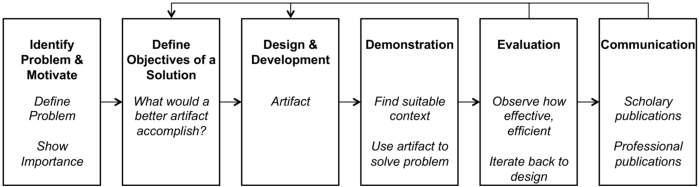
\includegraphics[width=.8\linewidth]{figures/DS-process}
	\caption{The Design Science Research process, adapted from~\cite{Peffers2008}}
	\label{fig:DS-process}
\end{figure}

%This doctoral thesis employs both design and behavioral science. Following the approach suggested by \cite{Berente2018}, real life data will be used for data-driven computationally-intensive theory development. \todoinline{JM: You really want to develop theory, or you aim to provide techniques? I think you work is more about providing technique - that are useful to inform the mentioned approach to theory building.} This approach can be seen as a combination between behavioral science and design science. The behavioral perspective is given by traditional theory development based on manual coding, e.g. \gls{gtm}. The design perspective is given by the creation of novel artifacts (e.g., software algorithms) that use trace data to automatically discover theory, e.g, \gls{ctd}. This thesis uses real world data gathered from the SHAPE project\footnote{\url{https://aic.ai.wu.ac.at/shape-project/}} and \gls{oss}. This data will be used both for generating propositions about process aspects and developing novel artifacts. These artifacts apply process mining methods to a new domain, also referred to as exaptation~\cite{Gregor2013}. 

%With reference to \gls{dsr} process in \Cref{fig:DS-process}, next sections show the design and development of the dataset and artifacts for addressing the requirements posed in \Cref{sec:problem-definition}.
%
%
%The following subsections explain the research method adopted in relation to \gls{dsr}. 

This proposal foresees the development of four different artifacts. These artifacts are interconnected to one another in that each of them tackles a different perspective of the overarching software development process. More specifically, each artifact is devised following the \gls{dsr} approach. These artifacts are useful useful to inform the mentioned approach to theory building \cite{Berente2018}.

Research rigor and validity are ensured by evaluating the artifacts with the \gls{feds}~\cite{Venable2016}. \Gls{feds} provides strategies for evaluating \gls{dsr} artifacts. More specifically, it takes into account two dimensions
\begin{inparaenum}[\itshape i)]
	\item the functional purpose of the
	evaluation (formative or summative); and 
	\item the paradigm of the evaluation (artificial or naturalistic).
\end{inparaenum} 
Moreover, it provides four steps for choosing an appropriate evaluation strategy
\begin{inparaenum}[\itshape i)]
	\item explicate the goals of the evaluation;
	\item choose the evaluation strategy or strategies
	\item determine the properties to evaluate; and
	\item design the individual evaluation episode(s). 
\end{inparaenum} 

Next, the evaluation strategies for each designed artifact are provided.


%% Please add the following required packages to your document preamble:
% \usepackage{booktabs}
% \usepackage[normalem]{ulem}
% \useunder{\uline}{\ul}{}
% \usepackage{longtable}
% Note: It may be necessary to compile the document several times to get a multi-page table to line up properly
\begin{longtable}[c]{@{}p{1cm}p{2.5cm}p{5cm}p{3cm}p{4cm}@{}}
\toprule
\textbf{Artifact} & \textbf{Features}                              & \textbf{Goals}                                                                                                                                                                                                                                                           & \textbf{Evaluation}                                                                                                                                  & \textbf{Iteration episodes}                                                                                                   \\* \midrule
\endhead
%
\bottomrule
\endfoot
%
\endlastfoot
%
\textbf{A1}       & time information                               & General goal: has to be applicable, usable, simple and provide overview as well as detailed view                                                                                                                                                                         & Quick and simple: the technique is directly evaluated with real data                                                                                 & First iteration (formative): initial design of gantt chart                                                                    \\
                  & duration of activities                         & Rigor: assured by the design science approach                                                                                                                                                                                                                            &                                                                                                                                                      & Second iteration: evaluation of successful identification of events and project structure                                     \\
                  & structure of the project                       & Uncertainty and risk reduction: artifacts is technically infeasible, data is unavailable                                                                                                                                                                                 &                                                                                                                                                      & Third iteration: run of the tool on real projects and provide a visualization                                                 \\
                  & granularity of events                          & Ethics: “big-brother is watching you” effect on people                                                                                                                                                                                                                   &                                                                                                                                                      &                                                                                                                               \\
                  &                                                & Efficiency: find all time patterns, algorithm runs in a reasonably short time                                                                                                                                                                                            &                                                                                                                                                      &                                                                                                                               \\* \midrule
\textbf{A2}       & difference between different instances of work & General goal: has to be applicable, usable, simple and provide overview as well as detailed view                                                                                                                                                                         & Quick and simple: the technique is firstly evaluated with a toy example, then revised and applied to a large number of software development projects & First iteration (formative): initial design of artifact and results  visualizations                                           \\
                  & amount of changes                              & Rigor: assured by the iterations                                                                                                                                                                                                                                         &                                                                                                                                                      & Second iteration: revision and choice of final visualization                                                                  \\
                  & handle unstructured data from comments         & Uncertainty and risk reduction: artifacts is technically infeasible adressed by developing by smaller iterations, data is unavailable addresses by local copy, results interpretation is hard addressed by mining processes from text                                    &                                                                                                                                                      & Third iteration: evaluation of efficacy on retrieving features                                                                \\
                  & evolutionary analysis of changes               & Ethics: n/a because data is public                                                                                                                                                                                                                                       &                                                                                                                                                      & Fourth iteration: run the technique on toy exampe (artificial evaluation). Validate efficacy and usefulness. Revise artifact. \\
                  & uncover work dependencies                      & Efficiency: find all work dependencies in a reasonable time                                                                                                                                                                                                              &                                                                                                                                                      & Firfth iteration: run the technique on real data sets from GitHub projects (naturalistic evaluation)                          \\* \midrule
\textbf{A3}       & determine roles of users                       & General goal: has to aplicable and provide correct classification of roles                                                                                                                                                                                               & Quick and simple: the technique is evaluated with real data from industry partners                                                                   & First iteration (formative): initial design of simple artifact voted to a simple and structured represenation of the data     \\
                  & handle user comments                           & Rigor: assured by the iterations                                                                                                                                                                                                                                         &                                                                                                                                                      & Second iteration: selection of features and classifiers traininig. Selection of the best features and classifiers.            \\
                  & automatically classify resources               & Uncertainty and risk reduction: risk is that artifact incorrectly classifies reources, this is reduced by using different training sets from industry partners and otaining feedback                                                                                     &                                                                                                                                                      & Third iteration: evaluation of results with real data from partners and feeback                                               \\
                  &                                                & Ethics: there is a risk of obtaining information about people’s work. This is mitigated by NDA signed by the parties involved                                                                                                                                            &                                                                                                                                                      &                                                                                                                               \\
                  &                                                & Efficiency: evaluated in terms of precision and recall                                                                                                                                                                                                                   &                                                                                                                                                      &                                                                                                                               \\* \midrule
\textbf{A4}       & handle comments from forum conversations       & General goal: has to aplicable to pull requests and provide informative and reliable process models about the generation of an idea                                                                                                                                      & Technical risk and efficacy: the technique is firstly evaluated with an initial dataset, then revised and evaluated with other projects              & First iteration (formative): initial exploratory analysis on the applicability of process mining techniques on pull requests  \\
                  & discover a process model                       & Rigor: assured by the iterations                                                                                                                                                                                                                                         &                                                                                                                                                      & Second iteration: evaluation of process mining methods and assessment of statistical significance of results                  \\
                  &                                                & Uncertainty and risk reduction: risks are: 1) activities of business processes are not mapped correctly – mitigated by manual annotation 2) the resulting model is not informative – mitigated by statistical techniques voted to cluster traces into significant groups &                                                                                                                                                      & Third iteration: mine process models that are statistically significant and analyze the idea generation patterns              \\
                  &                                                & Ethics: n/a. Only data from open source repositories will be used                                                                                                                                                                                                        &                                                                                                                                                      &                                                                                                                               \\
                  &                                                & Efficiency: the artifact can deal with complex projects quickly                                                                                                                                                                                                          &                                                                                                                                                      &                                                                                                                               \\* \bottomrule
\end{longtable}

\paragraph{Artifact A1.} 
~\\\noindent\rule[1ex]{2.5cm}{2pt}~\\	

Design objectives of \textbf{A1} are \begin{iiilist}
	\item has to be applicable, 
	\item usable, 
	\item simple and,
	\item provide overview as well as detailed view.
\end{iiilist} 
The following features are included: 
\begin{iiilist}
	\item time information,
	\item duration of activities,
	\item structure of the project, and
	\item roll-up and drill-down on granularity of events.
\end{iiilist}
Evaluation goals are 
\begin{iiilist}
\item rigor,
\item uncertainty and risk reduction,
\item ethics, and
\item efficiency.
\end{iiilist}
They are respectively addressed as follows. Rigor is assured by the design science approach. Uncertainty involves technical infeasibility and unavailability of the data. Infeasibility risk is reduced by starting from the design of small artifacts with basic features and incrementally improve. Unavailability risk is reduced by replication of the dataset locally. An ethics problem may regard the “big-brother is watching you” effect on people. This will be solved considering only data from partners and public repositories. Efficiency is evaluated by measuring whether all time patterns are found in a reasonably short time.

This artifact is evaluated through a Quick \& Simple strategy (see \cite{Venable2016}), i.e., the technique is directly evaluated with real data. This will include three iteration episodes 
	\begin{iiilist}
		\item initial design of Gantt chart (formative)
		\item evaluation of successful identification events, their duration and project structure; and 
		\item run of the tool on real projects and provide a visualization (summative).
	\end{iiilist}



\paragraph{Artifact A2.} 
%Addresses RQ2.
~\\\noindent\rule[1ex]{2.5cm}{2pt}	

Design objectives of \textbf{A2} include applicability, simplicity and providing comparison of different cases. The following features are designed: 
	\begin{iiilist}
		\item difference between work instances;
		\item measure of work: amount of changes;
		\item handle unstructured data from comments;
		\item evolutionary analysis of files; and
		\item uncover work dependencies.
	\end{iiilist}
Evaluation goals are as follows. Rigor is assured by the iterations. Uncertainty and risk reduction consist in: technical infeasibility -- addressed through development by smaller iterations, data unavailability -- addressed by local replication of data, and simplicity of results -- addressed by exploiting user comments and derive informative process labels. Ethics problems do not arise as the data for this artifact is already public on GitHub. Efficiency is evaluated by finding all work dependencies in a reasonable time. 

This artifact is evaluated through a Technical risk \& Efficacy strategy (see \cite{Venable2016}), i.e., the technique is firstly evaluated with a toy example, then revised and applied to a large number of software development projects. Five iteration episodes are included: 
	\begin{iiilist}
		\item initial design of artifact and results  visualizations(formative);
		\item revision and choice of final visualization;
		\item evaluation of efficacy on retrieving features;
		\item run the technique on toy example (artificial evaluation), validate efficacy and usefulness, revise artifact; and
		\item run the technique on real data sets from GitHub projects (summative and naturalistic evaluation).
	\end{iiilist}



\paragraph{Artifact A3.}
~\\\noindent\rule[1ex]{2.5cm}{2pt}

Design objectives of \textbf{A3} include applicability and correct classification of roles. The following features are designed 
	\begin{iiilist}
		\item determine roles of users;
		\item handle user comments; and
		\item automatically classify resources.
	\end{iiilist}
Evaluation goals are as follows. Rigor is assured by the iterations. Uncertainty and risk reduction regard classification. Incorrect resource classification risk is reduced by using different training set data from industry partners and obtaining feedback. An ethics risk is about obtaining information about people's work. This is mitigated by NDAs signed by the parties involved. Efficiency is evaluated in terms of precision and recall. 

This artifact is evaluated through a Quick \& Simple strategy (see \cite{Venable2016}), i.e., the technique is evaluated with real data from industry partners. Three iteration episodes are included: 
	\begin{iiilist}
		\item initial design of the artifact voted to a simple and structured representation of the data (formative)
		\item exploration and selection of the best features and classifiers.
		\item evaluation of results with real data from partners and feedback (summative + naturalistic).
	\end{iiilist}

\paragraph{Artifact A4.} 
%Addresses RQ2.
%\rule{3cm}{1pt}
~\\\noindent\rule[1ex]{2.5cm}{2pt}

Design objectives of \textbf{A4} are its applicability to pull requests and its functionality to provide informative and reliable process models about specific work patterns. The following features are designed.
	\begin{iiilist}
		\item handle comments from forum conversations, and
		\item discover a process model.
	\end{iiilist}
Evaluation goals are considered as follows. Rigor is assured by the iterations. Uncertainty and risk reduction the following
\begin{iiilist}
	\item activities of business processes are not mapped correctly -- mitigated by manual annotation; and
	\item the resulting model is not informative -- mitigated by statistical techniques voted to cluster traces into significant groups.
\end{iiilist} Ethics problems do not arise because only data from open source repositories will be used. Efficiency is measured by the extent to which the artifact can deal with complex projects quickly.

This artifact is evaluated through a Technical risk \& Efficacy strategy (see \cite{Venable2016}), i.e., the technique is firstly evaluated with an initial well-known dataset, then revised and evaluated with other projects. Three iteration episodes are included: 
	\begin{iiilist}
		\item initial exploratory analysis on the applicability of process mining techniques on pull requests (formative);
		\item evaluation of process mining methods and assessment of statistical significance of results; and
		\item mine process models that are statistically significant and analyze the idea generation patterns (summative + naturalistic).
	\end{iiilist}
%\end{description}



%Many scenarios in SHAPE require for automated solutions to respond to compliance problems. Compliance is regulated by rules and guidelines as for instance the European standards EN50126, EN50128, EN50129. These standards specify procedures and technical requirements for the development of programmable electronic systems that are used in railway control and protection applications. Thus, there is a clear need for transparency in the work that is done to make sure that it complies to the standards procedures. To this end, engineering projects are systematically verified by auditors who check if everything is done according to the rules imposed by the standards. This is typically done a posteriori and the challenge here is to able to understand all the process steps and their quality by looking at existing documentation. 
%It intends to support project managers or auditors who must validate the compliance of the work against existing rules and regulations. This involves building new artifacts in order to both partially automate compliance checking and help by providing better overviews on the existing process. 

%\begin{figure}
%	\centering
%	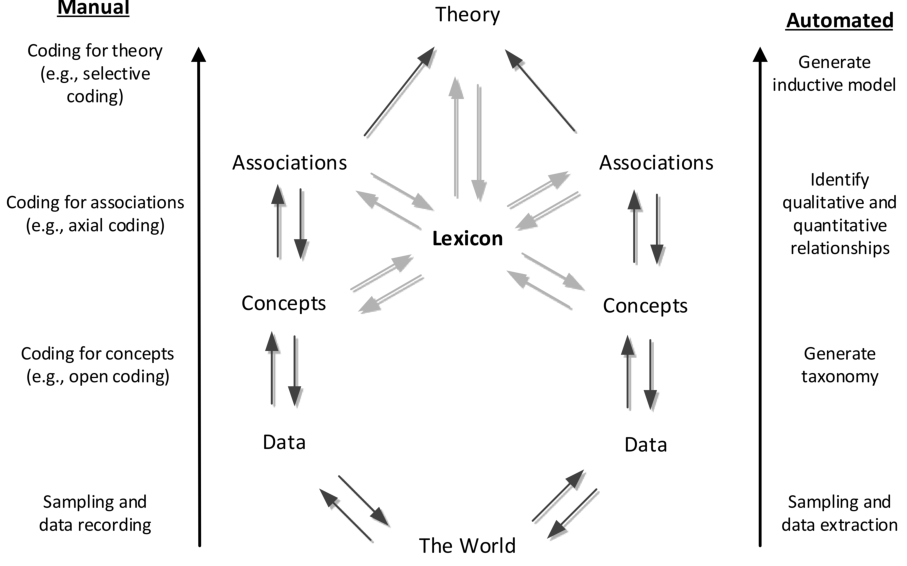
\includegraphics[width=0.7\linewidth]{figures/empirically-driven-theory-generation-1}
%	\caption{Empirically driven theory generation~\cite{Berente2018}}
%	\label{fig:empirically-driven-theory-generation}
%\end{figure}


%\begin{description}
%	\item[Guideline 1 -- Design as an Artifact.] Design-science research must produce a viable artifact in the form of a construct, a model, a method, or an instantiation In my research, I use state-of-the-art techniques and develop new artifacts that allow to capture information from both structured and unstructured types of data. 
%	
%	\item[Guideline 2 -- Problem Relevance.] The objective of design-science research is to develop technology based solutions to important and relevant business problems. My research takes inspiration from real world needs which include human-centric safety-critical automated solutions in the railway domain.  
%	
%	\item[Guideline 3 -- Design Evaluation.] The utility, quality, and efficacy of a design artifact must be rigorously demonstrated via well-executed evaluation methods. The real world scenarios that I encounter in the SHAPE project require for novel solutions, which involve the design of new algorithms. Algorithms are converted to operational software. This operational software is an instantiated artifact~\cite{Gregor2013}, which is then tested against real data. 
%	
%	\item[Guideline 4 -- Research Contributions.] Effective design-science research must provide clear and verifiable contributions in the areas of the design artifact, design foundations, and/or design methodologies. The contribution of my research can be positioned as a set of \emph{exapted} methods (cf. \gls{dsr} knowledge contribution framework~\cite{Gregor2013}) from the fields of process mining and text mining, which contribute to a better understanding of projects. 
%	
%	\item[Guideline 5 -- Research Rigor.] Design-science research relies upon the application of rigorous methods in both the construction and evaluation of the design artifact. My research builds upon existing work from natural language processing~\cite{de2006generating,Corro2013,klein2003accurate}, a number of \gls{vcs} mining works~\cite{Banitaan2015,Allamanis2013,Vasilescu2015,Karimi2016,German2015}, and process mining.
%%	\cite{van2011process,rubin2007process,Rubin2014a,rubin2014agile}. 
%I plan to adopt mature methods from the mentioned works and construct my artifacts upon existing ones. 
%	
%	\item[Guideline 6 -- Design as a Search Process.] 
%	The search for an effective artifact requires utilizing available means to reach desired ends while satisfying laws in the problem environment. I plan to build my artifacts based on state-of-the-art methods and technology and follow both a rigorous process as the one described in~\cite{Peffers2008} (cf. \cref{fig:DS-process}). Given the nature of my data, an exploratory phase may be required in the initial activity of this process. This may involve exploratory data analysis, as described in the data science process~\cite[p.~41]{Schutt2013}
%	
%	\item[Guideline 7 -- Communication of Research.] Design-science research must be presented effectively both to technology-oriented as well as management-oriented audiences. I will use guidelines~\cite{Gregor2013,Recker2015} in order to properly position my work. The main target will be \gls{bpm} conferences and journals. 
%	
%\end{description}


\subsection{Data Collection}

This thesis includes the collection of and generation of datasets from real life software projects. These project data were collected both from industrial partners and from \gls{oss}. \Cref{tab:dataset} summarizes the available data. Logs from industrial partner are concerned with specific development activities (e.g., building railway interlocking-system software) and include a sufficient number of events that cover one software release. Logs from \gls{oss} were manually extracted by GitHub repositories. A tool has then been devised to parse these data and use them to populate a database. An original dataset is represented by Github pull requests. This dataset contains a list of manually annotated pull requests using the coding scheme by \cite{Majchrzak2016}. An additional output of this thesis will be the creation of a larger dataset using a machine learning approach that is able to automatically categorize pull requests in the classes given by \cite{Majchrzak2016}.

% Please add the following required packages to your document preamble:
% \usepackage{booktabs}
\begin{table}[h]
\centering
\caption{Available dataset}
\label{tab:dataset}
\begin{tabular}{@{}lp{11cm}@{}}
%\toprule
\textbf{Log} & \textbf{Description} \\ \midrule
SHAPE & Industry \gls{vcs} from software development in the railway domain \\
Github & Logs from real world \gls{oss} development \\
Github pull requests & Manually annotated pull requests from one real life open source project \\
Jira & Log data from \gls{its} from industry partner \\
Asana & Generated dataset from project management tool of industrial partner \\
Kibana & Event traces from distributed process-agnostic enviroment used to handle communication among several processes \\ \bottomrule
\end{tabular}
\end{table}

\subsection{Expected Outcome}

In addition to an original dataset, this doctoral thesis is expected to produce outcomes that help the project manager analyze his software development processes. To this end new approaches in the form of artifacts~\cite{Peffers2008} will be devised. These artifacts will serve as proofs-of-concept for the applicability of the research. In particular, the artifacts must address each of the four process aspects. Therefore, the outcome is categorized according to the research questions derived in \Cref{sec:problem-definition} as follows.

\begin{itemize}	
	\item \textbf{Artifact A1: Mining the Time Perspective (RQ1)}. Novel technique that allows for gaining transparency on the time perspective of software development work.	For instance, and artifact that explicits what are the durations of tasks and when are actual tasks executed.
	
	\item \textbf{Artifact A2: Mining the Case Perspective (RQ2)}. Novel technique that allows for gaining transparency on the case perspective of software development work. For instance, an artifact that explicits how the different cases are handled and whether there is any dependency of work that might influence the case execution. 
	
	\item \textbf{Artifact A3: Mining the Organizational Perspective (RQ3)}. Novel technique that allows for gaining transparency on the organizations aspect of software development work. For instance, an artifact that explicits which are the actual roles software developers are covering and which is the organizational network. 
	
	\item \textbf{Artifact A4: Mining the Control-Flow Perspective (RQ4)}. Novel technique that allows for gaining transparency on the control-flow perspective of software development work. For instance, an artifact that allows for abstracting from data which is order of activities that are executed to accomplish a certain task or goal in software development.	
\end{itemize}

\Cref{fig:big-solution} shows the overall information coming from combining the four perspectives into a Gantt chart that is more informative to managers. 

\begin{figure}[]
	\centering
	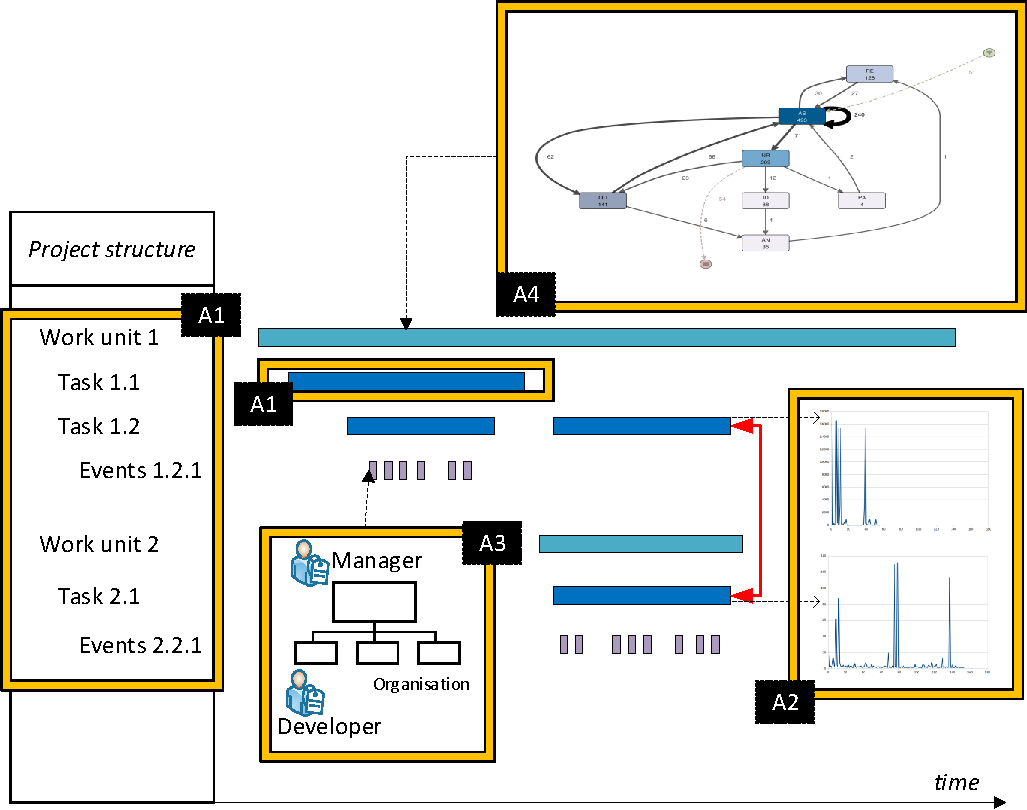
\includegraphics[width=\linewidth]{figures/big-solution2-crop.pdf}
	\caption{The empirical Gantt chart of software development. The four process perspectives combined.}
	\label{fig:big-solution}
\end{figure}


\section{Preliminary Results} \label{sec:preliminary-results}

Next, I present efforts done towards addressing the requirements presented in \Cref{sec:problem-definition}.

\subsection{A1. Mining the Time Perspective (RQ1)}

Mining the time perspective from a software repository is defined as extracting temporal process knowledge. This problem relates to monitoring whether the process was executed respecting a predefined plan. Typically the process involves various actors which track their work through the use of \gls{vcs}. Often, the plans are not represented in standard process notation. Rather, Gantt or PERT charts are used. 

\begin{figure}[h]
	\centering
	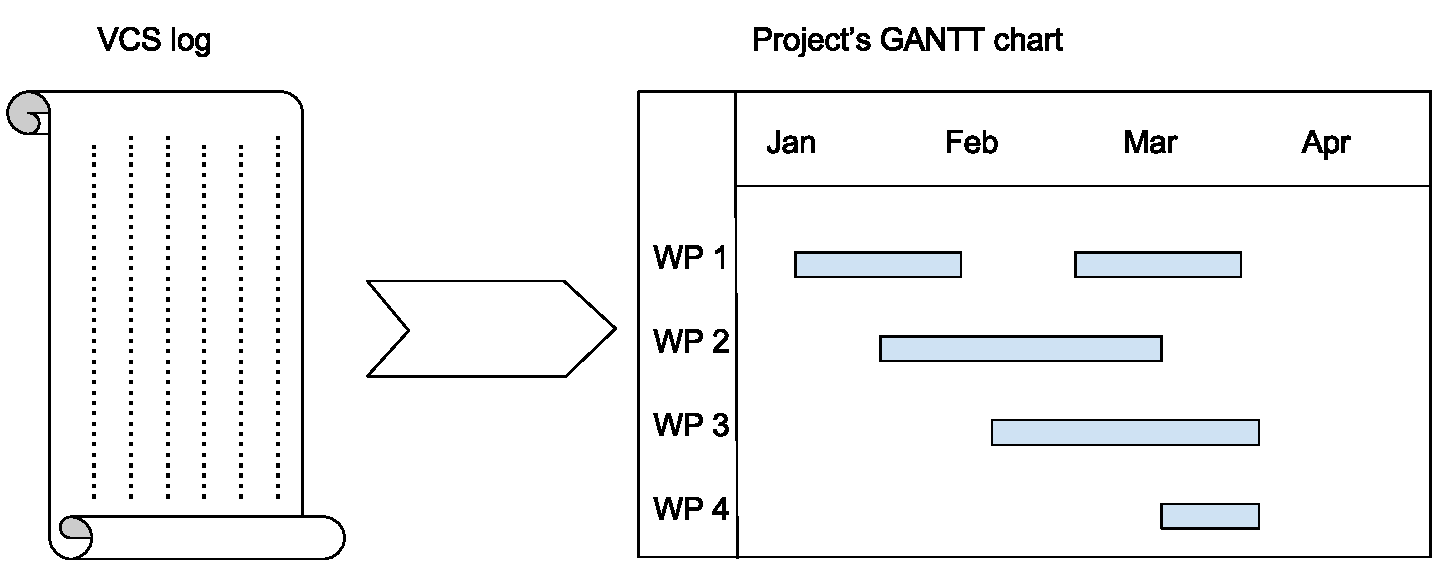
\includegraphics[width=0.6\linewidth]{figures/VCS-log-to-Gantt}
	\caption{Mining the time perspective of software development into a Gantt chart}
	\label{fig:vcs-log-to-gantt}
\end{figure}

Challenges are 
\begin{inparaenum}[\itshape i)]
	\item \emph{time approximation} (i.e., when the activity really started, compared to when it was registered in the log);
	\item \emph{granularity} (i.e., be able to switch from a detailed view of the single events and a coarse-grained view of the overall project); and
	\item \emph{coverage} (i.e., how much work effort was put within the duration of the activity).
\end{inparaenum} 
\Cref{fig:vcs-log-to-gantt} depicts the idea of mining a Gantt chart from \gls{vcs} logs. The output is presented in a way that is informative to project managers. Details about the technique can be found in~\cite{Bala2015}. 

\subsection{A2. Mining the Case Perspective (RQ2)}

The identification of process cases is not an easy task when it comes to software development data. However, a highly informative case candidate can be considered the data artifact itself. According to~\cite{VanderAalst2016b}, cases can also be characterized by the values of data elements. In line with this, it is possible to devise techniques that study the \emph{artifact evolution}. Although it can be input to process mining techniques, this evolution can also be analyzed as a time series. An example of such evolution is given in \Cref{fig:time-series1}, which shows the \gls{loc} changes over time.

\begin{figure}[h]
	\centering
	\begin{subfigure}[b]{.4\textwidth}
		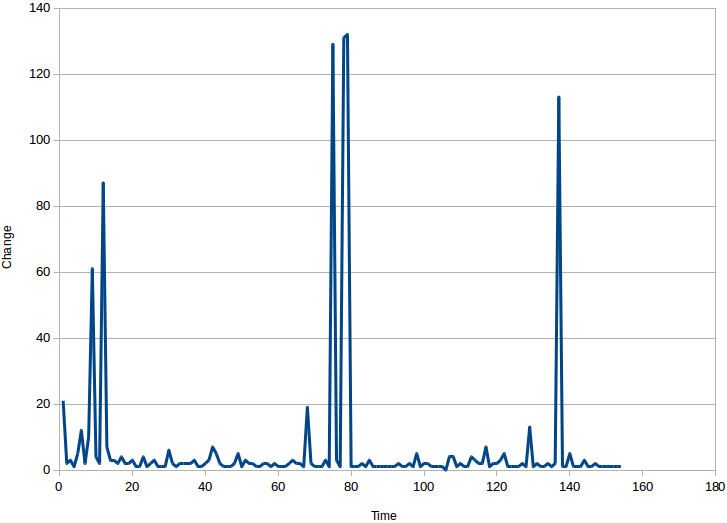
\includegraphics[width=\linewidth]{figures/time-series1}
	\end{subfigure}~
	\begin{subfigure}[b]{.4\textwidth}
		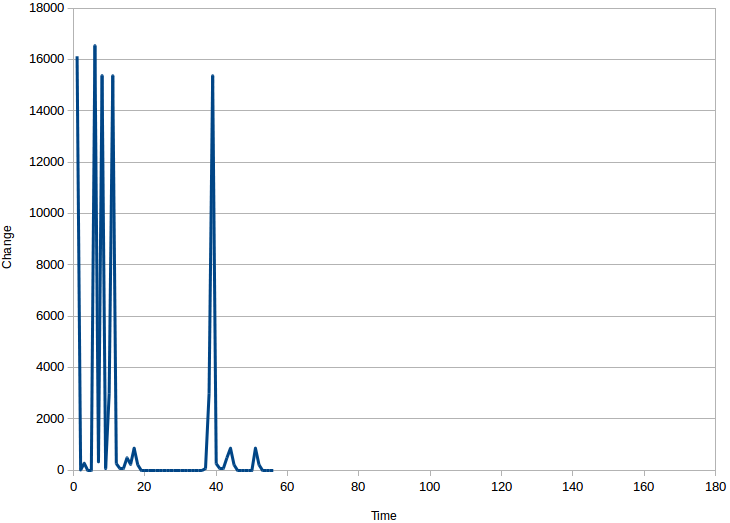
\includegraphics[width=\linewidth]{figures/time-series2}
	\end{subfigure}	
	\caption{Evolution of files in a version control systems: LOC changes over time}
	\label{fig:time-series1}
\end{figure}


Challenges related to the artifact evolution pertain \emph{prediction} of plateaus and \emph{pattern recognition}. The results reflect work patterns over the artifact. For example, when a data file is not being modified anymore, its time series has a plateau and it can be interpreted that the document is now ready for release. 
A relevant problem in software development is bad modularization. Especially, the dependency of two artifacts on one another is considered a bad practice. Two time series can be compared together and file dependencies can be found that reflect work coupling. This is equivalent to finding dependence between two processes which might have been designed for different purposes. 
\begin{figure}[h]
	\begin{subfigure}[b]{\textwidth}
		\centering
		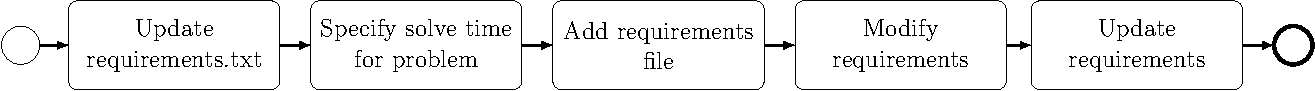
\includegraphics[width=\linewidth]{figures/requirementsTxtProcess}
		%		\caption{Evolution of file \texttt{requirements.txt}}
		\label{subfig:requirements-file-process}
	\end{subfigure}
	\begin{subfigure}[hb]{\textwidth}
		\centering
		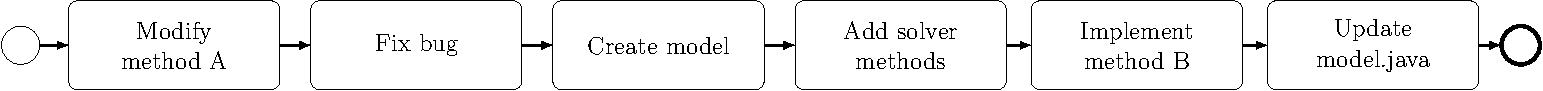
\includegraphics[width=\linewidth]{figures/modelProcess}
		%		\caption{Evolution of file \texttt{model.java}}
		\label{subfig:model-file-process}
	\end{subfigure}
	\caption{Processes of two work-dependent files. They may seem different but they co-evolve in time and space, i.e., they describe the same \emph{case}.}
	\label{fig:evaluated-processes}
\end{figure}

We have devised a proof-of-concept in~\cite{Bala2017a}. \Cref{fig:evaluated-processes} shows a possible outcome of the technique. The result is obtained by identifying couples of files with similar evolution and mining a business process from the comments. As the result is aggregated, several comments have been combined together and mined as a story. Among other things, the technique allows to profile existing software development projects.

\subsection{A3. Mining the Organizational Perspective (RQ3)}

Software development projects are knowledge intensive, thus involve creativity and flexibility. Project participants are free to tackle development tasks according to their expertise and ideas to solve ad-hoc problems. De facto, members may behave according several roles in the organization. Therefore, the discovery of \emph{de facto} roles within a software project may give important insights on the actual project. Role discovery can help with monitoring existing projects in two ways. First, emerging roles can be analyzed in order to have a better skills profiling of the resources. Second, emerging roles can be used to check whether resources are breaking contractual agreements or norms.

%There are works in \gls{msr} that can give good insights about social aspects behind software repositories~\cite{Teixeira2015}. Furthermore, \gls{nlp} techniques can be used to extract information from unstructured data, such as user comments. 

We have developed an approach for tackling the problem of mining the organizational perspective in software development projects. The approach provides information about the actors involved in the business process and their relations. In substance, it provides automatic classification of resources into company roles (e.g., developer, tester, etc) based on the comments of project participants. It works on \gls{vcs} logs and provides information about the people, their roles, other systems involved, the organization hierarchy, the social network, and resource profiling. \Cref{fig:infinica-resources} shows an example of resource profiles automatically inferred from \gls{vcs} comments.

\begin{figure}[]
	\centering
	\begin{subfigure}[b]{.4\textwidth}
		\centering
		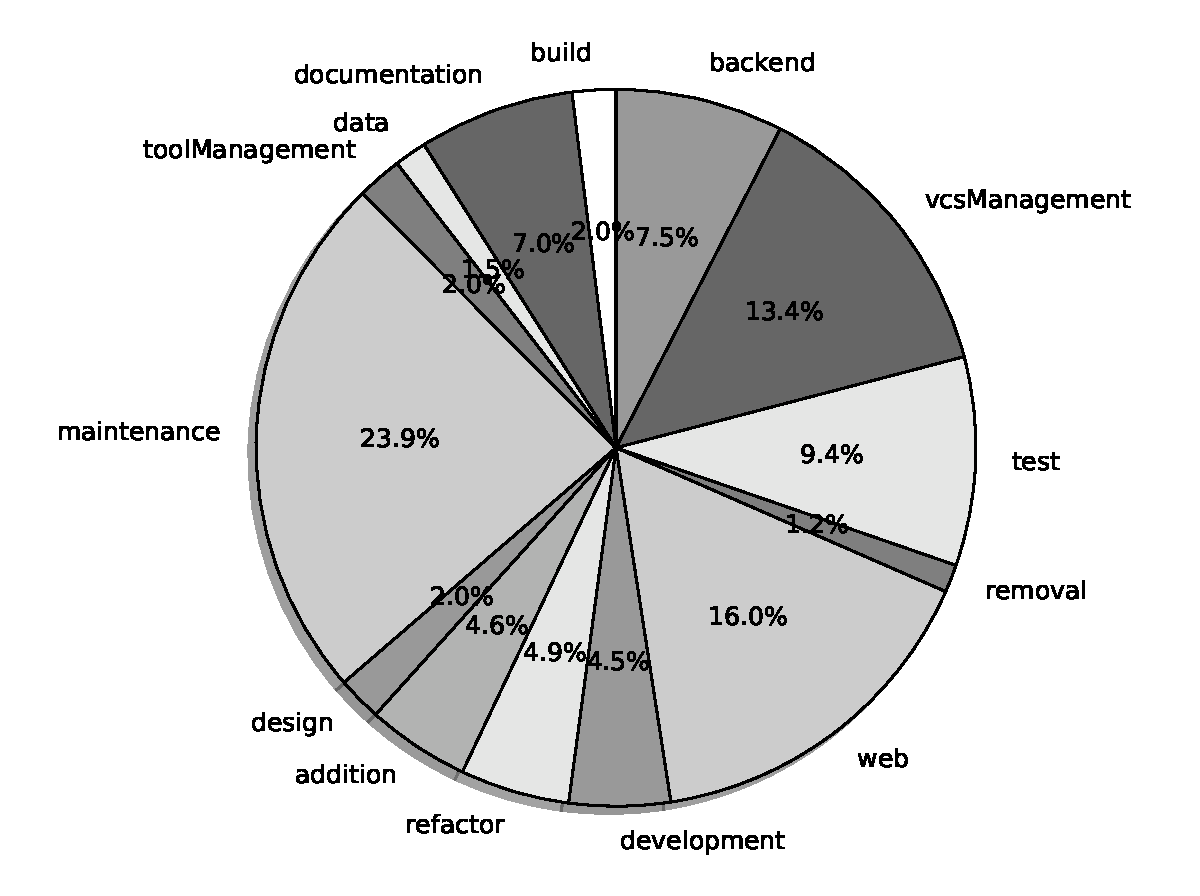
\includegraphics[width=\linewidth]{figures/infinica_developer.pdf}
		%		\caption{Evolution of file \texttt{requirements.txt}}
		%		\label{subfig:requirements-file-process}
	\end{subfigure}~
	\begin{subfigure}[b]{.4\textwidth}
		\centering
		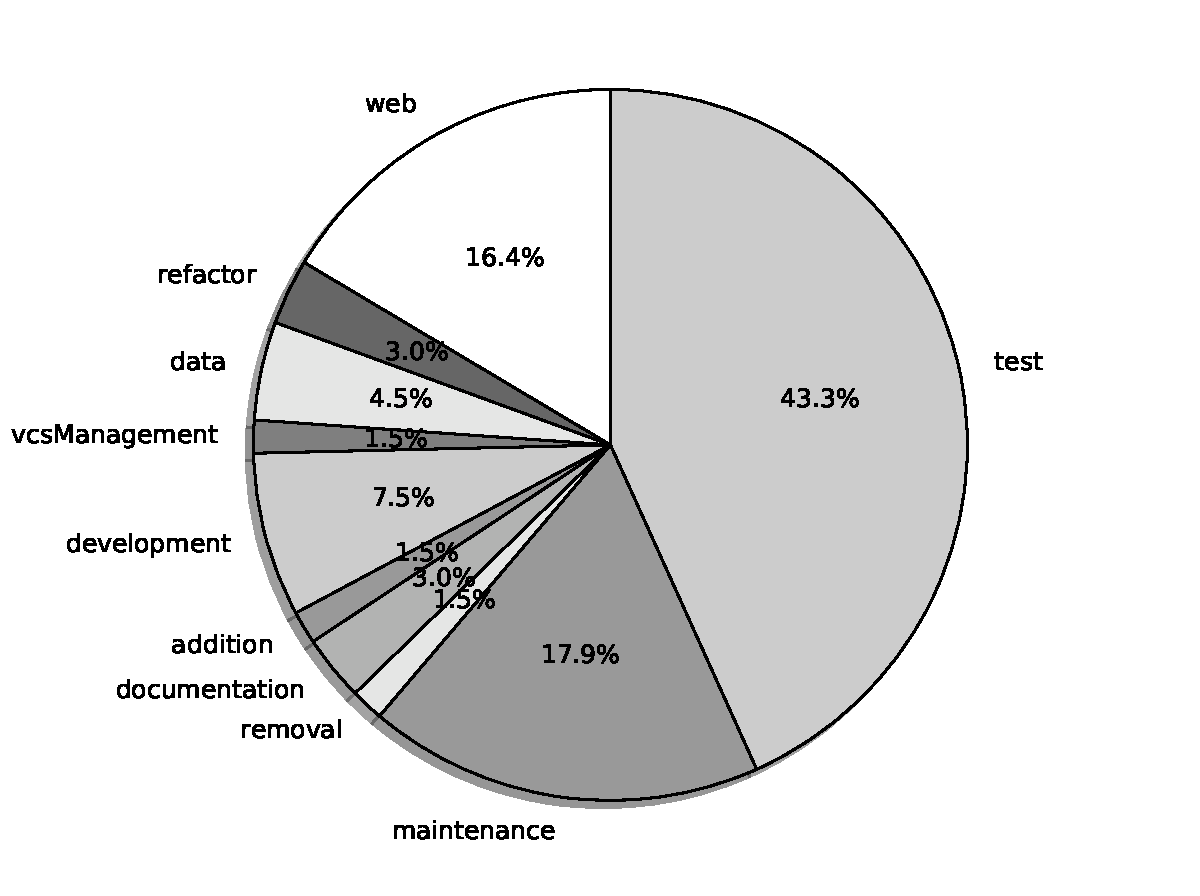
\includegraphics[width=\linewidth]{figures/infinica_tester.pdf}
		%		\caption{Evolution of file \texttt{model.java}}
		%		\label{subfig:model-file-process}
	\end{subfigure}
	\caption{Profiles of a developer and a tester, from left to right.}
	\label{fig:infinica-resources}
\end{figure}

Challenges of using \gls{nlp} concern the \emph{jargon} used by software developers. They often use technical terms, very short phrases, or a number of codes and hyperlinks. These makes \gls{nlp} techniques score low results even on simple tasks like sentence parsing, or name-entity recognition. Therefore, approaches should take into account several factors when mining for the organizational perspective. 
The result allows the manager to have measurable information about the resources. For example, do two people work better together and how can we build the best team? Details of the approach to extract resource profiles can be found in~\cite{Agrawal2016}. 

\section{Next Steps and Finalization of the Thesis}
\label{sec:next-steps}

\subsection{A4. Mining the Control-Flow Perspective (RQ4)}

Knowledge of the control flow of a software development process can be extracted from \gls{vcs} and \gls{its}. One important mechanism widely used in software development for collaboration are \emph{pull requests}. A pull request is issued every time a developer wants to contribute to the main source with a new piece of code. Pull requests trigger communication among different people and may help shedding light into problems, learn new things and obtain new ideas on the existing software. It is interesting for project managers and developers to better understand factors and behavior that makes a pull request successful. 

In ongoing work, we are investigating the relation of the pull request process and surrounding factors such as the generation of new ideas or change of behavior. We have obtained a data set of pull requests spanning over two years from an real world repository. User conversations have been manually annotated with codes that classify them into categories of comments. We are current able to discriminate whether a comment is a new idea, an assumption, a merge that closes a pull request, etc. Considering the pull request identifiers as cases and the codes as activities, we are able to extract the process of the pull requests. It is interesting to compare how the conversation (i.e., behavioral perspective) unfolds before and after a pull request is merged. We plan to explain these differences by also taking into account further information from text such as emotions. 


The challenge of mining the control-flow usually pertains the completeness of data and the case and activity identification. While \gls{pm} contribution have been focusing mostly on the control-flow perspective, techniques from \gls{msr} hardly go beyond mining the bug lifecycle~\cite{Akbarinasaji2018a}. The nature of software development process makes it difficult to recognize recurrent activities when only \gls{vcs} are analyzed. 

\subsection{Finalization of the Thesis}

The expected result for the above-mentioned work is an artifact that is able to explicitly show what are process patterns that lead to the generation of an idea. This will serve as a proof-of-concept that event data from projects can be used to increase understanding of process flow perspective. The overall thesis will be finalized by evaluating the results both against the real world dataset and project managers. There is ongoing work in which a questionnaire has been answered by industry partners. Questions pertains activities, tools and habits within a software development company. These information can be used to evaluate the artifacts developed by this thesis.

\section{Dissertation Relevance and Publication Plan}
\label{sec:dissertation-relevance}

\subsection{Implications for Research}

This proposal presents research on mining the software development process.
Approaches towards discovering the perspectives of time, resources and cases
have been developed and the results suggest that obtaining process knowledge
from software repositories brings new useful insights for the project managers.
Ongoing work aims to complete the research by tackling the problem of
discovering the flow-perspective of the software development process. Usefulness
will be evaluated through user studies.
This research extends the process mining field towards its adoption on software
repositories. Project managers would benefit from this research by having a
process perspective on their ongoing projects through visual models and diagrams,
thus overcoming existing flat approaches based on simple indicators such as
burndown charts or change plots offered by existing tools.

\subsection{Work Plan and Dissemination}
\Cref{fig:phd-plan} summarizes the work plan based on the artifacts to be build for addressing the four research questions. In other words, the thesis work is currently in its final stage, which involves the creation of artifact \textbf{A4} to address the corresponding research question \textbf{RQ4}. 

\begin{figure}[]
	\centering
	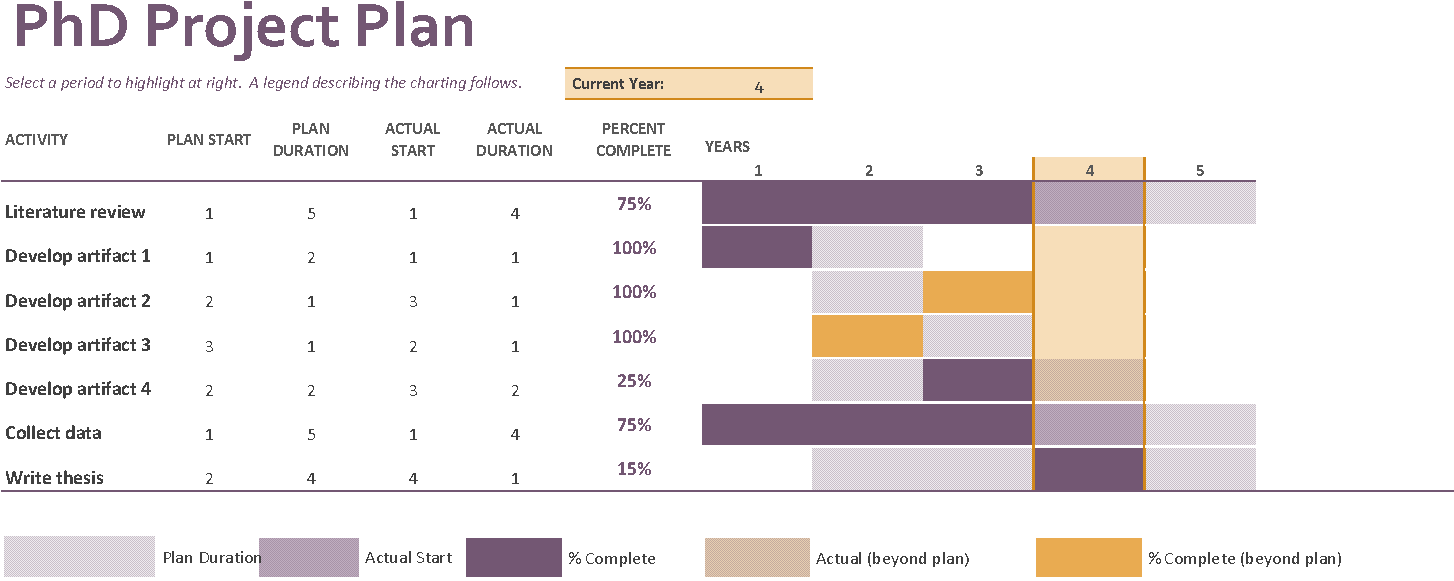
\includegraphics[width=\linewidth]{figures/PhD-plan-crop}
	\caption{Gantt chart of PhD Plan}
	\label{fig:phd-plan}
\end{figure}

Target venues for communicating the results are \gls{bpm} and software engineering journals and conferences.  
So far, the following publications have been achieved that directly address the research questions concerning time, organization, case and control-flow, as defined in \Cref{sec:problem-definition}.\\


\noindent {Mining the Time Perspective (\textbf{RQ1}):}
	
	\begin{itemize}
	\item \textbf{Bala, S.}, Cabanillas, C., Mendling, J., Rogge-Solti, A., and Polleres, A.: \textit{Mining Project-Oriented Business Processes}. In Hamid Reza Motahari-Nezhad, Jan Recker, and Matthias Weidlich, editors, BPM 2015, Innsbruck, Austria, volume 9253 of Lecture Notes in Computer Science, pages 425--440. Springer, 2015. \cite{Bala2015}
	\end{itemize}

\noindent {Mining the Case Perspective (\textbf{RQ2}):}

\begin{itemize}
	\item \textbf{Bala, S.}, Revoredo, K., de A.R. Gonçalves, J.C., Baião, F., Mendling, J., Santoro, F.: \textit{Uncovering the Hidden Co-evolution in the Work History of Software Projects}. In: Carmona, J., Engels, G., and Kumar, A. (eds.) Business Process Management - 15th International Conference, BPM 2017, Barcelona, Spain, September 10-15, 2017, Proceedings. pp. 164--180. Springer (2017). \cite{Bala2017a}
\end{itemize}

\noindent {Mining the Organizational Perspective (\textbf{RQ3}):}

\begin{itemize}
	\item Agrawal, K., Aschauer, M., Thonhofer, T., \textbf{Bala, S.}, Rogge-Solti, A., Tomsich, N.: \textit{Resource Classification from Version Control System Logs}. In: Proceedings - IEEE International Enterprise Distributed Object Computing Workshop, EDOC Workshop. pp. 249--258 (2016). \cite{Agrawal2016}
\end{itemize}


\noindent Publications that address the requirements in \Cref{sec:problem-definition} indirectly.


\begin{itemize}
	
	\item \textbf{Bala, S.}, Cabanillas, C., Haselböck, A., Havur, G., Mendling, J., Polleres, A., Sperl, S., Steyskal, S.: \textit{A Framework for Safety-Critical Process Management in Engineering Projects}. In: Ceravolo, P. and Rinderle-Ma, S. (eds.) Data-Driven Process Discovery and Analysis- SIMPDA. pp. 1--27. Springer (2015). \cite{Bala2017c} -- Related to \textbf{RQ1} \& \textbf{RQ3}.
	
	\item \textbf{Bala, S.}, Havur, G., Sperl, S., Steyskal, S., Haselböck, A., Mendling, J., Polleres, A.: SHAPEworks: A BPMS extension for complex process management. In: CEUR Workshop Proceedings. pp. 50--55 (2016). \cite{Bala2016} -- Related to \textbf{RQ1} \& \textbf{RQ3}.
	
\end{itemize}

\noindent Doctoral consortium and vision paper presenting the concepts of this research proposal.

\begin{itemize}
	\item \textbf{Bala, S.}: \textit{Mining projects from structured and unstructured data}. In: CEUR Workshop Proceedings (2017). \cite{Bala2017b}

	\item \textbf{Bala, S.}, Mendling, J.: \textit{Monitoring the Software Development Process
		with Process Mining}. In Boris Shishkov, editor, Business Modeling and Software
	Design, volume 319 of Lecture Notes in Business Information Processing, 2018 \cite{Bala2018} 
	
\end{itemize}

\noindent From ongoing work the following publications are expected.

\begin{itemize}
	\item Case study on tool productivity. Collaboration with researchers from the University of Ljubljana to be submitted to a class A journal on information systems. -- Related to \textbf{RQ1}, \textbf{RQ3} and \textbf{RQ4}.
	
	\item Process mining pull requests for identifying idea-creation patterns. Collaboration with researchers from Stevens Institute of Technology to be submitted to a class A journal on information systems. -- Related to \textbf{RQ4}.
	
	\item Mining knowledge intensive processes from pull requests. Collaboration with researchers from Federal University of the State of Rio de Janeiro (UNIRIO) to be submitted to a class A conference. -- Related to \textbf{RQ2} \& \textbf{RQ4}.
	
\end{itemize}

\noindent Other work in the \gls{bpm} area.

\begin{itemize}
	\item Woli\'nski, B., \textbf{Bala, S.}: \textit{Comprehensive Business Process Management at Siemens: Implementing Business Process Excellence}. In: vom Brocke, J. and Mendling, J. (eds.) Business Process Management Cases: Digital Innovation and Business Transformation in Practice. pp. 111--124. Springer International Publishing, Cham (2018). \cite{Wolinski2018}
\end{itemize}

\addcontentsline{toc}{section}{References}
\bibliographystyle{alpha}
\bibliography{bib/Bala,bib/Bibliography}

\end{document}
